\documentclass[12pt,a4paper,oneside]{book}
%-------------------------------------------------------------------
\usepackage[utf8]{inputenc}
\usepackage{vietnam}
\usepackage{amsfonts}
\usepackage{latexsym, amsmath, amsxtra, amssymb, amscd, amsthm,fancyhdr} %, txfonts, pxfonts}
\usepackage[top=2.5cm, bottom=2.5cm, left=2.7cm, right=2cm]{geometry}
\usepackage{indentfirst} %thụt lề dòng đầu tiên
\usepackage{graphicx} % chèn ảnh,
\usepackage{algorithm} %1 chèn thuật toán
\usepackage{algpseudocode} %2 chèn thuật toán
\setcounter{secnumdepth}{4} % subsubsubsection
\usepackage{placeins} % để sử dụng \FloatBarrier cố định vị trí
\usepackage{subfigure} % chèn hình phụ
\usepackage{pdfpages} % chèn pdf vào luận văn
\usepackage{tabularx} % chèn bảng
\usepackage{multirow} % bảng có thể gộp hàng hoặc cột
\usepackage{hyperref} % cite papers, trinh tu build f6 f11 f6 f1
\usepackage{pgf,tikz,pgfplots} % hình từ geogebra
\usetikzlibrary{arrows} % hình từ geogebra
\pgfplotsset{compat=1.5} % hình từ geogebra gốc là 1.15
\usepackage{mathrsfs} % hình từ geogebra
\usepackage{fancyhdr} % header và footer
\usepackage{caption} % không hiện 1 table or figure in list of t, f
\usepackage{makecell} % xuong hang trong 1 cell table

% Set up------------------------------------------------------------
\renewcommand{\baselinestretch}{1.5} %khoảng cách giữa các dòng
\setlength{\parskip}{0.5em} %khoảng cách giữa các đoạn
\numberwithin{equation}{chapter} % đánh số công thức theo chapter
\numberwithin{figure}{chapter} % đánh số hình theo chapter
\numberwithin{table}{chapter} % đánh số bảng theo chapter
\renewcommand{\algorithmicrequire}{\textbf{Input:}} %thay require trong algorithmic thanh Input
\renewcommand{\algorithmicensure}{\textbf{Output:}} %thay ensure trong algorithmic thanh Output

\pagestyle{fancy}
\fancyhf{}
\rhead{\fontsize{10pt}{0pt}{\selectfont{\leftmark}}}
\rfoot{\fontsize{10pt}{0pt}{\selectfont{SVTH: Nguyễn Thành Đạt}}}
\cfoot{\thepage}
%\rfoot{\fontsize{10pt}{0pt}{\selectfont{GVHD: PSG.TS Hà Hoàng Kha}}}
\renewcommand{\headrulewidth}{0.5pt}
\renewcommand{\footrulewidth}{0.5pt}

\fancypagestyle{loi_cam_doan}{\fancyhf{}
\rhead{\fontsize{10pt}{0pt}{\selectfont{LỜI CAM ĐOAN}}}
\rfoot{\fontsize{10pt}{0pt}{\selectfont{SVTH: Nguyễn Thành Đạt}}}
\cfoot{\thepage}
%\rfoot{\fontsize{10pt}{0pt}{\selectfont{GVHD: PGS.TS Hà Hoàng Kha}}}
\renewcommand{\headrulewidth}{0.5pt}
\renewcommand{\footrulewidth}{0.5pt}
}

\fancypagestyle{loi_cam_on}{\fancyhf{}
\rhead{\fontsize{10pt}{0pt}{\selectfont{LỜI CẢM ƠN}}}
\rfoot{\fontsize{10pt}{0pt}{\selectfont{SVTH: Nguyễn Thành Đạt}}}
\cfoot{\thepage}
%\rfoot{\fontsize{10pt}{0pt}{\selectfont{GVHD: PGS.TS Hà Hoàng Kha}}}
\renewcommand{\headrulewidth}{0.5pt}
\renewcommand{\footrulewidth}{0.5pt}
}

\fancypagestyle{tom_tat}{\fancyhf{}
\rhead{\fontsize{10pt}{0pt}{\selectfont{TÓM TẮT}}}
\rfoot{\fontsize{10pt}{0pt}{\selectfont{SVTH: Nguyễn Thành Đạt}}}
\cfoot{\thepage}
%\rfoot{\fontsize{10pt}{0pt}{\selectfont{GVHD: PGS.TS Hà Hoàng Kha}}}
\renewcommand{\headrulewidth}{0.5pt}
\renewcommand{\footrulewidth}{0.5pt}
}

\fancypagestyle{abstract}{\fancyhf{} %
\rhead{\fontsize{10pt}{0pt}{\selectfont{ABSTRACT}}}%
\rfoot{\fontsize{10pt}{0pt}{\selectfont{SVTH: Nguyễn Thành Đạt}}}
\cfoot{\thepage}
%\rfoot{\fontsize{10pt}{0pt}{\selectfont{GVHD: PGS.TS Hà Hoàng Kha}}}
\renewcommand{\headrulewidth}{0.5pt}
\renewcommand{\footrulewidth}{0.5pt}
}

\fancypagestyle{danhmucviettat}{\fancyhf{}
\rhead{\fontsize{10pt}{0pt}{\selectfont{DANH MỤC VIẾT TẮT}}}
\rfoot{\fontsize{10pt}{0pt}{\selectfont{SVTH: Nguyễn Thành Đạt}}}
\cfoot{\thepage}
%\rfoot{\fontsize{10pt}{0pt}{\selectfont{GVHD: PGS.TS Hà Hoàng Kha}}}
\renewcommand{\headrulewidth}{0.5pt}
\renewcommand{\footrulewidth}{0.5pt}
}

\fancypagestyle{phuluc}{\fancyhf{}
\rhead{\fontsize{10pt}{0pt}{\selectfont{PHỤ LỤC}}}
\lfoot{\fontsize{10pt}{0pt}{\selectfont{SVTH: Nguyễn Thành Đạt}}}
\cfoot{\thepage}
%\rfoot{\fontsize{10pt}{0pt}{\selectfont{GVHD: PGS.TS Hà Hoàng Kha}}}
\renewcommand{\headrulewidth}{0.5pt}
\renewcommand{\footrulewidth}{0.5pt}
}

\begin{document}
%\fontsize{13pt}{13pt}\selectfont
\newcolumntype{L}[1]{>{\raggedright\arraybackslash}p{#1}} % có thể định nghĩa kich thước cho bảng
\newcolumntype{C}[1]{>{\centering\arraybackslash}p{#1}}
\newcolumntype{R}[1]{>{\raggedleft\arraybackslash}p{#1}}

\begin{titlepage}

\newcommand{\HRule}{\rule{\linewidth}{0.5mm}}
% \renewcommand{\baselinestretch}{2.0}
\centering

\large ĐẠI HỌC QUỐC GIA THÀNH PHỐ HỒ CHÍ MINH \\
TRƯỜNG ĐẠI HỌC BÁCH KHOA \\
KHOA ĐIỆN - ĐIỆN TỬ  \\
BỘ MÔN VIỄN THÔNG  \\ [0.8cm]

\begin{figure}[!ht]
    \centering
    
\includegraphics[scale=0.3]{front_pages/Logo_BK.png}
    \label{fig:logo}
\end{figure}

\bfseries
\Large{LUẬN VĂN TỐT NGHIỆP ĐẠI HỌC} \\[1.3cm]

\LARGE{NHẬN DẠNG NGÔN NGỮ KÝ HIỆU CHO NGƯỜI KHIẾM THÍNH SỬ DỤNG KỸ THUẬT HỌC SÂU: TÁCH VÀ PHÂN TÍCH ĐẶC TRƯNG KHUNG XƯƠNG TRÊN VIDEO RGB} \\ [2.1cm]

\normalfont
\normalsize
% \small
\begin{tabular}{r l}
    \fontsize{14pt}{0pt}{\selectfont{GVHD:}} & \fontsize{14pt}{0pt}{\selectfont{PGS.TS HÀ HOÀNG KHA}} \\
    \fontsize{14pt}{0pt}{\selectfont{SVTH:}} & \fontsize{14pt}{0pt}{\selectfont{NGUYỄN THÀNH ĐẠT - 1510698}}  					
                        
\end{tabular} 
\\ [2.1cm]

TP. HỒ CHÍ MINH, THÁNG 12 NĂM 2019
% \vfill
\end{titlepage}


%------------------------------------------------------------------
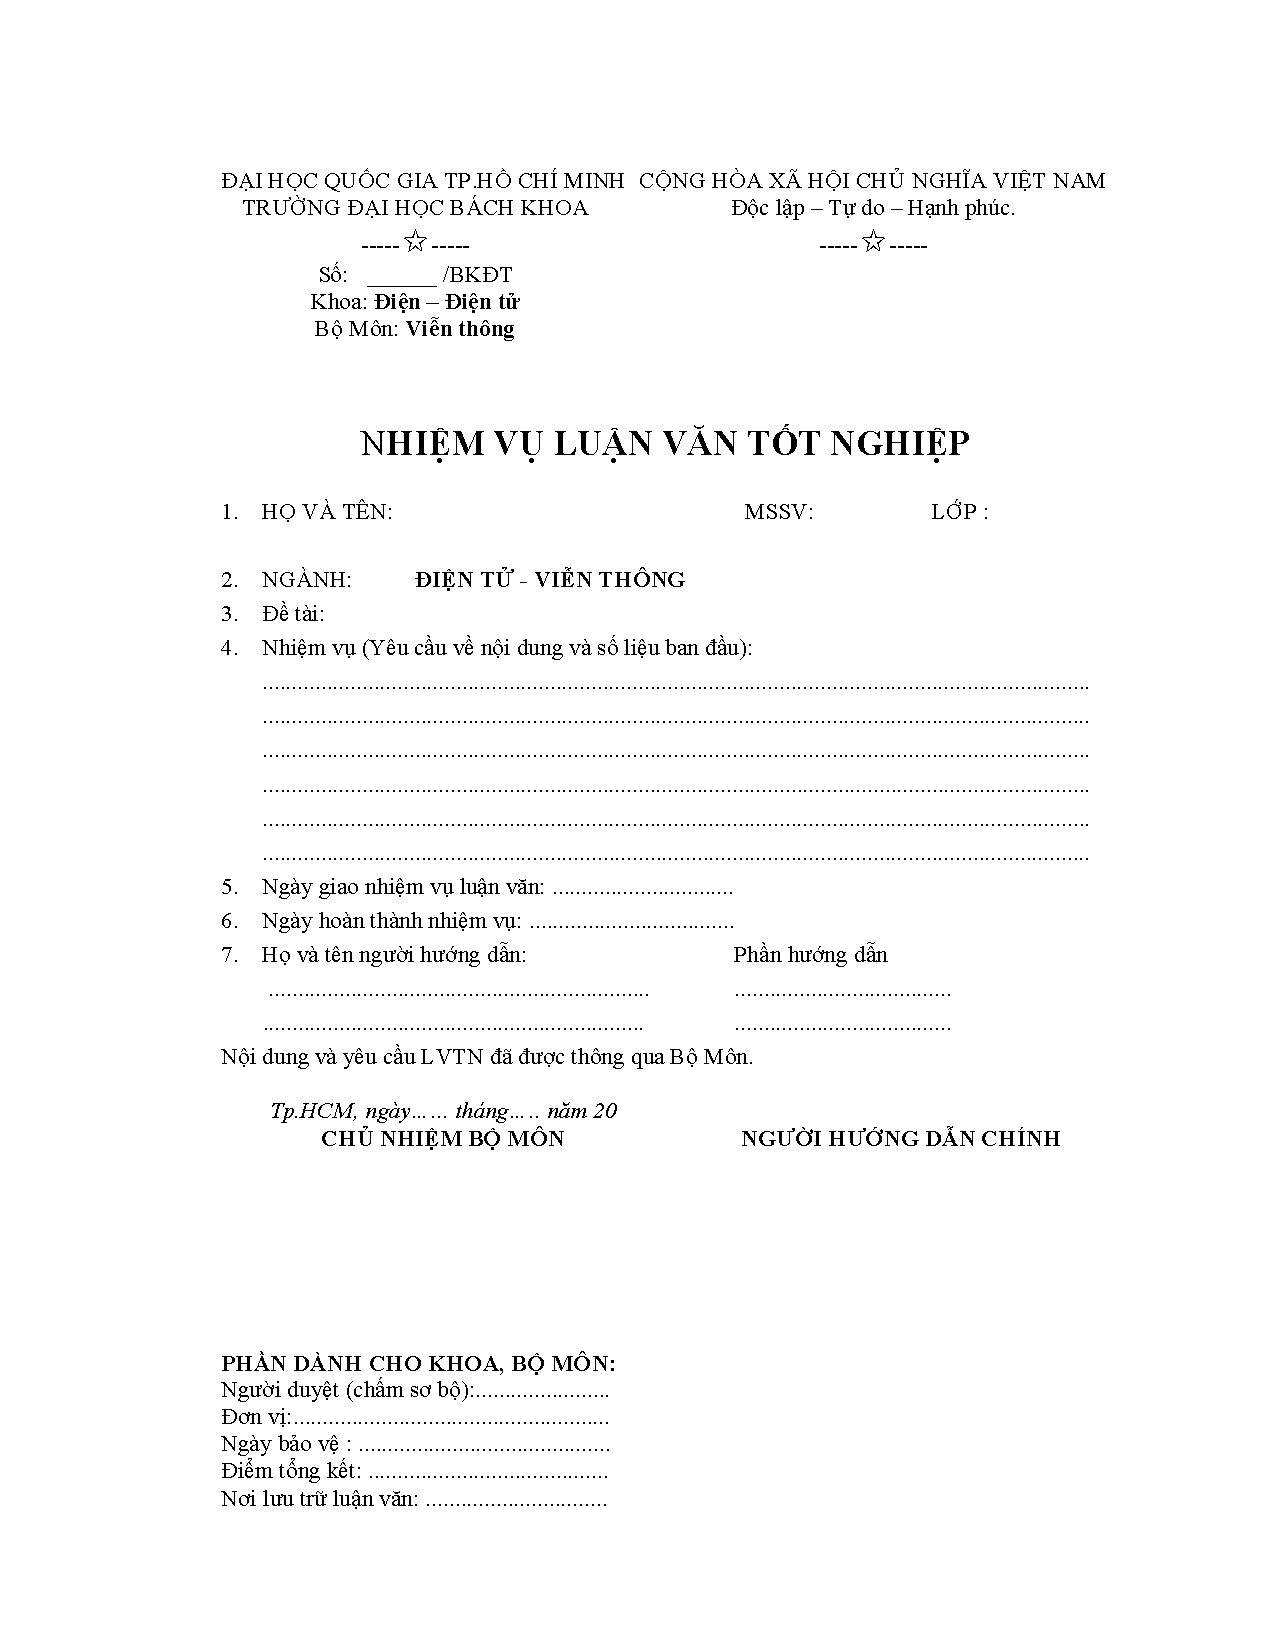
\includepdf[pages=-]{front_pages/nhiem_vu_lv.pdf}

%------------------------------------------------------------------
\newpage
\pagenumbering{roman}
\addcontentsline{toc}{chapter}{LỜI CẢM ƠN}
\thispagestyle{loi_cam_on}
\begin{center}
{\fontsize{18pt}{30pt}{\selectfont{\textbf{Lời cảm ơn}}}}
\end{center}

\textit{Trong thời gian thực hiện luận án này, em đã nhận được sự hỗ trợ nhiệt tình, hướng dẫn tận tình và những lời động viên tích cực từ các giảng viên, bạn bè và gia đình. Do đó, em đã hoàn thành luận án như mục tiêu đã đặt ra. Những lời giảng dạy quý báu, không những về mặt kiến thức mà còn về đạo đức làm người của các quý thầy cô sẽ là hành trang cho con đường tương lai của các thế hệ sinh viên.}

\textit{Em xin gửi đến thầy Hà Hoàng Kha, giảng viên hướng dẫn trực tiếp đề tài, lời biết ơn sâu sắc. Thầy đã dành thời gian quý báu để gặp gỡ, thảo luận, đưa ra những vấn đề hay để rèn luyện chúng tôi khả năng giải quyết vấn đề. Thầy là người đã theo tường bước đi của chúng tôi, tận tình chỉ bảo, hướng dẫn chúng tôi từ khi làm đồ án, đề cương cho đến luận văn. Ngoài những kiến thức chuyên ngành, chúng tôi còn nhận được những lời khuyên, kinh nghiệm quý giá trong học tập và nghiên cứu từ thầy.}

\textit{Em cũng xin cảm ơn chân thành đến cha mẹ đã động viên và tạo điều kiện giúp đỡ chúng tôi vượt qua những khó khăn trong suốt quá trình học tập và nghiên cứu.}

\textit{Mặc dù đã cố gắng trong phạm vi và khả năng cho phép, nhưng luận văn không thể tránh khỏi những thiếu sót, rất mong được sự góp ý của quý thầy cô và các bạn.}

\textit{Cuối cùng, xin chân thành cảm ơn quý thầy cô và các bạn đã dành thời gian đọc luận văn này.}


%------------------------------------------------------------------
\newpage
\addcontentsline{toc}{chapter}{LỜI CAM ĐOAN}
\thispagestyle{loi_cam_doan}
\begin{center}
{\fontsize{18pt}{30pt}{\selectfont{\textbf{Lời cam đoan}}}}
\end{center}

\noindent Em xin cam đoan rằng, luận văn tốt nghiệp "Nhận dạng ngôn ngữ ký hiệu cho người khiếm thính sử dụng kỹ thuật học sâu: tách và phân tích đặc trưng khung xương trên video RGB" là công trình nghiên cứu của em dưới sự hướng dẫn của PGS.TS Hà Hoàng Kha. Đề tài xuất phát từ nhu cầu thực tiễn và nguyện vọng muốn thực hiện của em. Ngoại trừ những nội dung được biên soạn lại từ các công trình khác đã ghi rõ, các nội dung, kết quả kiểm tra đánh giá thực nghiệm trình bày trong luận văn này là kết quả nghiên cứu do chính em thực hiện, hoàn toàn không phải sao chép từ bất kỳ một tài liệu hoặc công trình nghiên cứu nào khác.

Nếu không thực hiện đúng các cam kết trên, chúng tôi xin hoàn toàn chịu trách nhiệm trước kỷ luật của nhà trường cũng như pháp luật Nhà nước.

\begin{flushright}
Sinh viên thực hiện
\end{flushright}


%------------------------------------------------------------------
\newpage
\addcontentsline{toc}{chapter}{TÓM TẮT}
\thispagestyle{tom_tat}
\begin{center}
{\fontsize{18pt}{30pt}{\selectfont{\textbf{Tóm tắt}}}}
\end{center}

Trong luận văn này, em đã thực hiện viết ứng dụng realtime nhận diện được một số từ ngữ thông dụng trong ngôn ngữ ký hiệu của người khiếm thính khi giao tiếp. Ứng dụng được xây dựng với mục đích giúp cho người khiếm thính giao tiếp dễ dàng hơn với người bình thường khi họ không hiếu ngôn ngữ ký hiệu của người khiếm thính.

Bởi những phát triển trong học máy và học sâu gần đây, đã giúp con người giải quyết được những bài toán thực tế mà trước đây tưởng chừng như máy tính không thể làm được. Trong ứng dụng này em đã sử dụng một trong các phương pháp học máy đó để giải quyết bài toán nhận diện ngôn ngữ ký hiệu cho người khiếm thính Việt Nam. Phương pháp nhận diện mà đề tài sử dụng chia làm 2 bước. Đầu tiên từ hình ảnh RGB có chứa hình ảnh người khiếm thính đang diễn tả một từ ngữ do camera truyền vào. Ứng dụng sử dụng một mạng CNN là mạng mobilenet để trích xuất đặc trưng khung xương là tọa độ các khớp xương trên ảnh 2D (tổng cộng có 18 khớp xương ban đầu). Sau đó các tọa độ khớp xương này được đưa vào một mạng DNN để từ đó phân loại ra các hành động diễn tả từ ngữ mà mạng đã học được. Cuối cùng ứng dụng xuất ra từ ngữ mà người đứng trước camera muốn diễn tả và xuất ra màn hình.

Phương pháp nhận diện dựa vào trích xuất đặc trưng khung xương là một phương pháp khá hay và lạ so với các nghiên cứu liên quan trước đây. Điểm hay của phương pháp này là việc trích xuất khung xương đã khái quát gần như toàn bộ tư thế và hành động mà người khiếm thị muốn diễn tả. Việc này còn làm giảm số chiều dữ liệu so với việc từ một hình ảnh RGB đưa vào để phân loại ra từ ngữ gì. Việc còn lại chỉ cần phân loại hành động dựa trên đặc trưng đã được trích xuất bằng một mạng DNN cấu trúc nhỏ. Việc này giúp tăng tốc độ xử lý của ứng dụng lên đáp ứng được việc xử lý realtime.

Các kết quả thực nghiệm thu được từ hệ thống cho thấy tỷ lệ nhận dạng cao và tốc độ đáp ứng đủ nhanh cho hoạt động chế độ thời gian thực.

%------------------------------------------------------------------
\newpage
\thispagestyle{abstract}
\begin{center}
{\fontsize{18pt}{30pt}{\selectfont{\textbf{ABSTRACT}}}}
\end{center}



\textbf{Key words:} 

%------------------------------------------------------------------
\newpage
\addcontentsline{toc}{chapter}{MỤC LỤC}
{\fontsize{12pt}{5pt}\selectfont
\tableofcontents}


%------------------------------------------------------------------
\newpage
\addcontentsline{toc}{chapter}{DANH SÁCH HÌNH VẼ}
\listoffigures


%------------------------------------------------------------------
\newpage
\addcontentsline{toc}{chapter}{DANH SÁCH BẢNG}
\listoftables


%------------------------------------------------------------------
\newpage
\thispagestyle{danhmucviettat}
\addcontentsline{toc}{chapter}{DANH MỤC VIẾT TẮT}
{\fontsize{18pt}{30pt}{\selectfont{\textbf{Danh mục viết tắt}}}}

\FloatBarrier
\begin{table}[h]
\centering
\captionsetup{list=no}
\begin{center}
\begin{tabularx}{\columnwidth}{XX}
NN & : Neural Network \\
CNNs & : Convolutional Neural Networks\\
DNN & : Deep Neural Network \\
DL & : Deep Learning \\
MLP & : Multi Layer Perceptron \\
SGD & : Stochastic Gradient Descent \\
SJM & : Skeleton Joints Mapping \\
PAFs & : Part Affinity Fields  \\
CFMs & : Confidence Maps

\end{tabularx}
\end{center}
\end{table}
\FloatBarrier

\newpage
\setcounter{page}{1}
\pagenumbering{arabic}
\chapter{TỔNG QUAN}
\label{s:tong_quan}
Nội dung chương đặt vấn đề tổng quan bài toán nhận dạng ngôn ngữ ký hiệu hiện nay và một số các công trình nghiên cứu về nhận dạng ngôn ngữ ký hiệu đã công bố trong nước và quốc tế. Từ đó đưa ra lý do chọn đề tài nhận dạng ngôn ngữ ký hiệu, giới thiệu về công cụ hỗ trợ cũng như mục tiêu, nhiệm vụ của đề tài cần tập trung giải quyết. Ngoài ra, chương mở đầu cũng giới thiệu phương pháp xử lý đề tài luận văn và trình bày bố cục nội dung trình bày xuyên suốt bài báo cáo.

\section{Đặt vấn đề}
Khiếm thính là trình trạng một người có thính giác kém, không nghe được những âm thanh, tiếng nói mà một người bình thường có thể nghe được. Theo số liệu thống kê năm 2014 của Trung tâm nghiên cứu Giáo dục đặc biệt (Viện Khoa học GD Việt Nam), Việt Nam có khoảng 7 triệu người khuyết tật, trong đó có hơn 1 triệu người khiếm thính. Do khả năng nghe bị suy giảm nên việc giao tiếp bằng lời nói ở cộng đồng người khiếm thính  và với người bình thường dường như là không thể. Để thay thế cho việc giao tiếp bằng tiếng nói, “ngôn ngữ ký hiệu” được ra đời nhằm phục vụ việc giao tiếp trực tiếp mà không cần thông qua lời nói.
Ngôn ngữ ký hiệu hay ngôn ngữ dấu hiệu, thủ ngữ là ngôn ngữ dùng những biểu hiện của bàn tay thay cho âm thanh của tiếng nói. Ngôn ngữ ký hiệu do người khiếm thính tạo ra nhằm giúp họ có thể giao tiếp với nhau trong cộng đồng của mình và tiếp thu tri thức của xã hội. Ngôn ngữ ký hiệu không như chữ viết tay hay lời nói có một cách thức và ngữ pháp cụ thể, ký hiệu rõ ràng để có thể mô hình hóa được. Để sử dụng ngôn ngữ ký hiệu, người giao tiếp cần thể hiện cử chỉ bằng cả bàn tay và cánh tay, kết hợp với điệu bộ của cơ thể để có thể diễn tả ý nghĩa mong muốn. Tuy được cộng đồng người khiếm thính sử dụng phổ biến nhưng đối với người bình thường, hầu như đa số đều không hiểu ngôn ngữ ký hiệu. Ngoài ra, ngôn ngữ ký hiệu giữa các nước trên thế giới, thậm chí giữa các vùng miền trong một nước cũng có sự khác nhau. Việc này khiến cho việc giao tiếp của người khiếm thính gặp rất nhiều khó khăn. Vì vậy một hệ thống nhận dạng ngôn ngữ ký hiệu tự động phiên dịch sang tiếng nói giúp người khiếm thính hòa nhập cộng đồng là thật sự cần thiết.
Với những lý do đó, trong đề cương này em xin trình bày một mô hình nhận dạng ngôn ngữ ký hiệu qua phân tích hình ảnh từ camera. Hệ thống này có khả năng quan sát, phát hiện con người và nhận diện hành động mà người đứng trước camera muốn diễn đạt. 

\section{Những nghiên cứu liên quan}
\label{ss:nghien_cuu_lien_quan}
Lĩnh vực xử lý, phân loại, nhận diện ngôn ngữ ký hiệu rất rộng và phức tạp do tính phong phú của chữ cái, câu từ và đặc tính không cấu trúc của các hành động con người. Các hướng phát triển trong lĩnh vực này rất tiềm năng và bùng nổ trong những năm gần đây.

Trên thế giới, đã có nhiều nghiên cứu phát triển các dịch vụ thông dịch ngôn ngữ ký hiệu và các sản phẩm công nghệ nhằm hỗ trợ người khiếm thính trong giao tiếp xã hội. Một số sản phẩm nổi bật như găng tay chuyển đổi ngôn ngữ ký hiệu thành giọng nói \cite{tl1}, các phần mềm dịch từ văn bản/ giọng nói sang ngôn ngữ ký hiệu hay các từ điển tra cứu ngôn ngữ ký hiệu online \cite{tl2}. Một số tác giả cũng đã nghiên cứu sử dụng thiết bị Kinect trong việc nhận dạng các con số và các ký tự chữ cái theo ký hiệu ngôn ngữ người câm \cite{tl3}, tuy nhiên việc nhận dạng là dựa trên ảnh tĩnh chưa có những giải pháp nhận dạng ảnh động theo như các ký hiệu hiệu ngôn ngữ tiếng Việt.

Ở các nước, các nhà nghiên cứu đã tiếp cận bài toán nhận dạng cử chỉ bàn tay theo rất nhiều hướng khác nhau như dựa vào màu sắc bàn tay, hình dáng bàn tay hay công trình của Viola $\&$ Jones dùng các đặc trưng Haarlike.

Ngoài ra, lĩnh vực nhận diện cử chỉ của con người được quan tâm và nghiên cứu trong rất nhiều năm từ năm 1992 \cite{Yamato} với giải thuật HMM của Junji YAMATO cho đến những năm gần đây, sử dụng phương pháp SVM cục bộ của Christian Schudlt vào năm 2004 \cite{Schuldt:2004:RHA:1018429.1020906}, và các phương pháp khác như: giải thuật khung xương \cite{Chen:2006:HAR:1178782.1178808}, \cite{Forsyth}, \cite{With}. Các bài khảo sát chi tiết có thể được tìm thấy ở \cite{Cristani201386} khảo sát cách thức nhận diện hành động con người và đưa ra chi tiết nhiều bài báo có thể tham khảo.

Như đã đề cập ở các phần trên, phương pháp SVM chỉ hoạt động tốt với các ảnh tĩnh, nên các nhận diện chính xác của SVM phải nói chính xác là các cử chỉ của con người tại thời điểm tức thời đó đã được nhận diện chính xác, không phải là một hành động gồm nhiều cử chỉ. Luận văn này bên cạnh SVM thì cũng tập trung nhiều vào HMM nên các bài báo liên quan đến SVM và HMM đều được xem xét kỹ, trong đó có một số phương pháp rất hay và có thể được xem xét:

\begin{itemize}
\item Xây dựng mô hình 3D dựa vào nhiều camera ở các vị trí khác nhau \cite{HLUT1}
\item Nhận diện hành động con người dựa trên mô tả các đặc trưng góc 3D \cite{6693448}
\item Sử dụng nhiều thiết bị được gắn trên người \cite{4650859}
\end{itemize}

Mặc dù đã được nghiên cứu trong thời gian dài, tuy nhiên do đặc điểm của việc nhận dạng hành động con người rất phức tạp và không có một cấu trúc rõ ràng dẫn đến việc rất khó áp dụng cho thực tế hoặc một lĩnh vực rộng rãi.

\section{Mục tiêu của luận văn}
\subsection{Tìm hiểu}
Để có thể thực hiện việc nhận dạng ngôn ngữ ký hiệu, cần xác định được phương pháp thực hiện, lựa chọn các giải thuật hợp lý phù hợp với điều kiện thực tế và khả năng có thể ứng dụng cao nhất.
Phương án thực hiện được lựa chọn ban đầu có 3 phương án: 

Phương án 1: sử dụng thiết bị kinect để trích xuất hình dáng khung xương sau đó nhận dạng ngôn ngữ ideoký hiệu bằng thuật toán Hidden Markov Model từ chuỗi ký tự khung xương được trích xuất ra.

Phương án 2: Thực hiện xây dựng mạng kết hợp Convoluntion Neural Network kết hợp với Long Short Term Memory để nhận dạng hành động từ video.

Phương án 3: Trích xuất hình dáng khung xương từ từng frame ảnh 2D bằng mạng CNN để xuất ra tọa độ khung xương trên hệ tọa độ 2D. Sử dụng một mạng Deep neural network để nhận dạng ngôn ngữ ký hiệu từ chuỗi khung xương đó.

Ở phương án 1 việc sử dụng thiết bị kinect sẽ là quá cồng kềnh để có thể mang theo, và sử dụng trong đời sống hàng ngày. Mô hình HMM có thể là một mô hình máy học cổ điển, còn nhiều nhược điểm hơn so với các mô hình mới hiện nay. Ở phương án 2, để phân loại hành động, cần có tập dữ liệu lớn vì với mỗi góc nhìn khác nhau sẽ cho ra một ảnh khác nhau và với cùng một hành động sẽ cho ra những đặc trưng khác nhau, như vậy sẽ khó để có thể xây dựng mô hình này. Phương án 3 được chọn vì có nhiều ưu điểm hơn phương án 1 và 2.

\subsection{Thực hiện}
Ứng dụng hướng tới hỗ trợ cộng đồng người người khiếm thính trong giao tiếp thường ngày nên việc đầu tiên cần hướng đến là tính tiện lợi và dễ sử dụng. Vì vậy thiết bị giúp hỗ trợ người khiếm thính cần có thể dễ dàng mang đi gọn nhẹ. Do đó mục tiêu luận văn hướng đến là thực hiện phần mềm để có thể hoạt động trên điện thoại thông minh. 


\section{Bố cục trình bày}
\label{ss:bo_cuc_trinh_bay}
Bố cục của luận văn sẽ được trình bày theo trình tự và những nội dung được khái quát trong bảng \ref{table:bo_cuc_luan_van}.

\FloatBarrier
\begin{table}[h]
\caption{Tổng quan các chương của luận văn}
\label{table:bo_cuc_luan_van}
\centering
\begin{center}
\begin{tabular}{|c|p{13cm}|} 
 \hline
Chương  & Nội dung \\
 \hline
 Chương 1 & Giới thiệu chung về ngôn ngữ ký hiệu; Các nghiên cứu về nhận dạng ngôn ngữ ký hiệu; sơ lược mục tiêu, tổng quan và cấu trúc các phần của luận văn.\\
 \hline 
 Chương 2 & Trình bày lý thuyết về học sâu, các thuật toán huấn luyện mạng và mạng mobile net.\\
 \hline 
 Chương 3 & Giới thiệu các nghiên cứu về ước lượng đặc trưng khung xương; Cách thức hoạt động của mạng ước tính đặc trưng khung xương mà luận văn sử dụng .\\
 \hline
 Chương 4 & Trình bày về mạng neural network được luận văn đề xuất để phân loại các từ trong ngôn ngữ ký hiệu; Cách xử lý dữ liệu đầu vào của mạng; cách huấn luyện mạng \\
 \hline 
 Chương 5 & Cách thức ứng dụng hoạt động.\\
 \hline
 Chương 6 & Các thử nghiệm, kết quả và đánh g.iá\\
 \hline
 Chương 7 & Tổng kết.\\
 \hline
 
\end{tabular}
\end{center}
\end{table}
\FloatBarrier



\newpage
\chapter{CƠ SỞ LÝ THUYẾT}
\label{c:co_so_ly_thuyet}

%\section{CÁC LÝ THUYẾT LIÊN QUAN ĐẾN HỌC SÂU}
%\label{s:ly_thuyet_hoc_sau}

\section{MẠNG NEURAL NETWOK}
Nguồn tham khao: https://dominhhai.github.io/vi/2018/04/nn-intro/

				https://ujjwalkarn.me/2016/08/09/quick-intro-neural-networks/
				
				https://towardsdatascience.com/machine-learning-for-beginners-an-introduction-to-neural-networks-d49f22d238f9
				
				http://cs231n.github.io/neural-networks-1/
Con chó có thể phân biệt được người thân trong gia đình và người lạ hay đứa trẻ có thể phân biệt được các con vật. Những việc tưởng chừng như rất đơn giản nhưng lại cực kì khó để thực hiện bằng máy tính. Vậy sự khác biệt nằm ở đâu? Câu trả lời nằm ở bộ não với lượng lớn các nơ-ron thần kinh liên kết với nhau. Thế thì máy tính có nên mô phỏng lại mô hình ấy để giải các bài toán trên ???

Neural là tính từ của neuron (nơ-ron), network chỉ cấu trúc đồ thị nên neural network (NN) là một hệ thống tính toán lấy cảm hứng từ sự hoạt động của các nơ-ron trong hệ thần kinh.

Mạng noron nhân tạo (Neural Network - NN) là một mô hình tính toán được lấy cảm hứng từ cách mạng noron sinh học trong não người xử lý thông tin. Kết hợp với các kĩ thuật học sâu (Deep Learning - DL), NN  trở thành một công cụ hiệu quả và có nhiều kết quả đột phá cho nhiều bài toán khó như nhận dạng ảnh, nhận dạng giọng nói thị giác máy tính và xử lý ngôn ngữ tự nhiên. Trong nội dung này, luận văn sẽ trình bày các lý thuyết cơ bản của mạng NN từ các thành phần cơ bản, kiến trúc mạng và các kỹ thuật huấn luyện (training) một mạng NN.

\subsection{Hoạt động của các neuron sinh học}

\FloatBarrier
\begin{figure}[htp]
\begin{center}
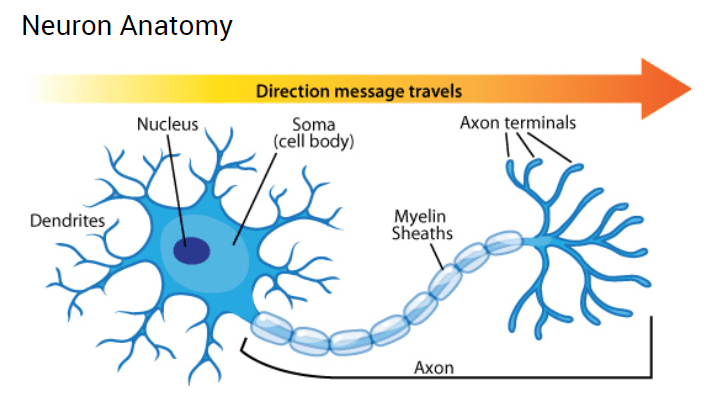
\includegraphics[scale=0.8]{chap2/c2_figs/neuron.png}
\end{center}
\caption{Cấu trúc một tế bào thần kinh}
\label{fig:neuronsinhhoc}
\end{figure}
\FloatBarrier
\centerline{Nguồn: https://askabiologist.asu.edu/neuron-anatomy}

Neuron là đơn vị cơ bản cấu tạo hệ thống thần kinh và là một phần quan trọng nhất của não. Não chúng ta gồm khoảng 10 triệu neuron và mỗi neuron liên kết với khoangr 10.000 neuron khác.

Ở mỗi neuron có phần thân (soma) chứa nhân, các tín hiệu đầu vào qua sợi nhánh (dendrites) và các tín hiệu đầu ra qua sợi trục (axon) kết nối với các neuron khác. Hiểu đơn giản mỗi neuron nhận dữ liệu đầu vào qua sợi nhánh và truyền dữ liệu đầu ra qua sợi trục, đến các sợi nhánh của các neuron khác.

Mỗi neuron nhận xung điện từ các neuron khác qua sợi nhánh. Nếu các xung điện này đủ lớn để kích hoạt neuron, thì tín hiệu này đi qua sợi trục đến các sợi nhánh của các neuron khác. => Ở mỗi neuron cần quyết định có kích hoạt neuron đấy hay không.

Tuy nhiên NN chỉ là lấy cảm hứng từ não bộ và cách nó hoạt động, chứ không phải bắt chước toàn bộ các chức năng của nó. Việc chính của chúng ta là dùng mô hình đấy đi giải quyết các bài toán chúng ta cần.

\subsection{Perceptron}
\label{s:perceptron}
\FloatBarrier
\begin{figure}[htp]
\begin{center}
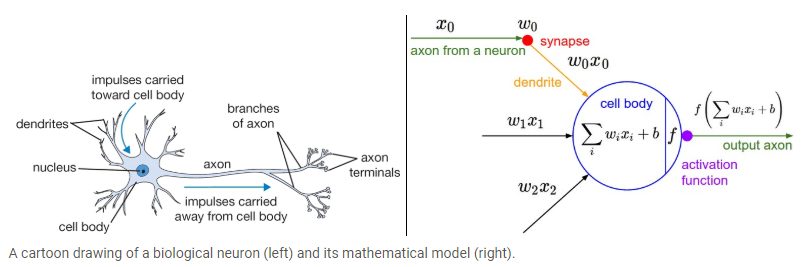
\includegraphics[scale=0.6]{chap2/c2_figs/perceptron.PNG}
\end{center}
\caption{Perceptron}
\label{fig:perceptron}
\end{figure}
\FloatBarrier

Lấy ý tưởng từ neuron sinh học, neuron nhân tạo với tên gọi perceptron cũng họat động theo cách gần giống với neuron sinh học để tạo thành một mạng thần kinh nhân tạo cho máy tính.

Đơn vị tính toán cơ bản trong một mạng NN được gọi là perceptron và thường được gọi là \textbf{node} hay \textbf{unit}. Một node nhận các đầu vào từ các nodes khác hoặc từ nguồn bên ngoài, sau đó tính toán tạo ra giá trị ngõ ra. Mỗi ngõ vào có một trọng số liên kết và giá trị này biểu thi mức độ liên quan giữa node hiện tại và node trước nó. Node áp dụng một hàm $f$ (được giới thiệu ở nội dung bên dưới) vào tổng các các tích ngõ vào và trọng số để tạo giá trị ngõ ra. Hình \ref{fig:single_neuron} miêu tả chi tiết một neuron và các hoạt động của nó.

\FloatBarrier
\begin{figure}[htp]
\begin{center}
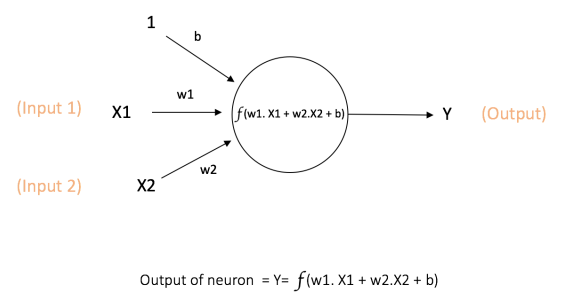
\includegraphics[scale=1]{chap2/c2_figs/single_neuron.PNG}
\end{center}
\caption{Một neuron cơ bản}
\label{fig:single_neuron}
\end{figure}
\FloatBarrier

Node trong hình \ref{fig:single_neuron} có hai đầu vào \textbf{Input 1} và \textbf{Input 2} có giá trị tương ứng $X1$ và $X2$, trọng số là \textbf{w1} và \textbf{w2}. Ngoài ra, có một đầu vào khác với giá trị \textbf{1} và trọng số b (được gọi là bias). Ngõ ra của node là Y được tính toán như hình \ref{fig:single_neuron}. Hàm \textbf{f} là hàm phi tuyến tính và được gọi là hàm kích hoạt (Activation Function). Đặc tính phi tuyến của hàm kích hoạt giúp mạng NN có thể "học" những dữ liệu thực trọng tự nhiên và hầu hết chúng đều có tính chất phi tuyến.

Các hàm kích hoạt thường được sử dụng trong thực tế:
\begin{itemize}
\item \textbf{Sigmoid:} lấy giá trị ngõ vào thực và ép nó nằm trong giới hạn [0, 1].
\begin{equation}
\sigma (x) = \frac{1}{{1 + {e^{ - x}}}}
\end{equation}
\item \textbf{Tanh:} lấy giá trị ngõ vào thực và ép nó nằm trong giới hạn [-1, 1].
\begin{equation}
\tanh (x) = 2\sigma (2x) - 1
\end{equation}
\item \textbf{ReLU:} lấy giá trị ngõ vào thực và lấy ngưỡng ở 0 (thay thế các giá trị âm bằng 0 hoặc giá trị rất nhỏ).
\begin{equation}
f(x) = \max (0,x)
\end{equation}
\end{itemize}

\noindent Đồ thị các hàm kích hoạt được mô tả trong hình \ref{fig:activation_function}.

\FloatBarrier
\begin{figure}[htp]
\begin{center}
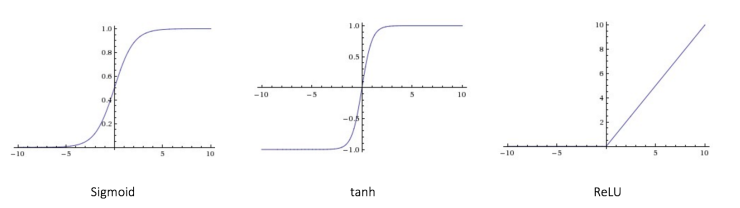
\includegraphics[scale=0.8]{chap2/c2_figs/activation_function.PNG}
\end{center}
\caption{Đồ thị các hàm kích hoạt}
\label{fig:activation_function}
\end{figure}
\FloatBarrier

Tầm quan trọng của bias: 

\subsection{Kiến trúc mạng Neuron Network}

Một mạng NN được xây dựng gồm nhiều lớp (layer). Mỗi lớp được cấu thành từ nhiều node cơ bản (đã trình bày trong mục \ref{s:perceptron}). Ngõ ra của các node ở lớp phía trước là ngõ vào của các node lớp phía sau, chúng được gọi là các liên kết (connection) và tương ứng với các trọng số khác nhau.

\FloatBarrier
\begin{figure}[htp]
\begin{center}
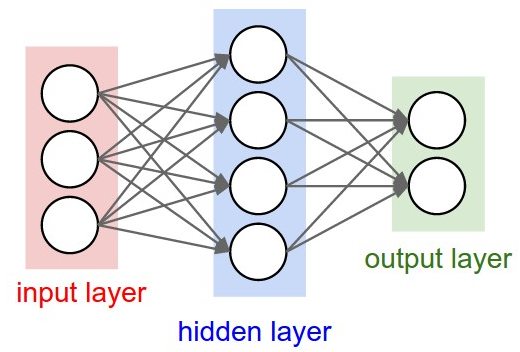
\includegraphics[scale=0.8]{chap2/c2_figs/structure_NN.PNG}
\end{center}
\caption{Mạng Neural Network cơ bản}
\label{fig:structure_NN}
\end{figure}
\FloatBarrier

Một mạng NN cơ bản sẽ có 3 tầng (minh họa trong hình \ref{fig:structure_NN}):
\begin{itemize}
\item \textbf{Tầng vào} (\textit{input layer}): Là tầng bên trái cùng của mạng thể hiện cho các đầu vào của mạng.
\item \textbf{Tầng ra} (\textit{output layer}): Là tầng bên phải cùng của mạng thể hiện cho các đầu ra của mạng.
\item \textbf{Tầng ẩn} (\textit{hidden layer}): Là tầng nằm giữa tầng vào và tầng ra thể hiện cho việc suy luận logic của mạng.
\end{itemize}

Một mạng NN chỉ có một tầng vào và một tầng ra, nhưng có thể có nhiều tầng ẩn. Số lượng tầng ẩn phụ thuộc vào độ phức tạp của bài toán được mạng NN giải quyết và được thiết kế dựa trên kinh nghiệm của người xây dựng mạng.

\subsection{Hoạt động của mạng}
\label{hoat_dong_cua_mang}

Tín hiệu đầu vào (gồm các thông tin cần dự đoán) sẽ được truyền từ input layer. Sau đó được tính toán qua các hidden layer bới các nodes. Cuối cùng output layer sẽ thực hiện việc dự đoán và phân lọai.\\

Mỗi node trong hidden layer và output layer sẽ thực hiện các công việc sau:
\begin{itemize}
\item Liên kết với tất cả các node ở layer trước đó với các hệ số $w$ riêng.
\item Mỗi node có 1 hệ số bias b riêng.
\item Diễn ra 2 bước: tính tổng linear và áp dụng activation function đưa ra output của node.
\end{itemize}

Để hiểu rõ ràng nhất, ta đi sâu vào các tính toán trong một mạng NN cụ thể như hình \ref{fig:NN}.\\

\FloatBarrier
\begin{figure}[htp]
\begin{center}
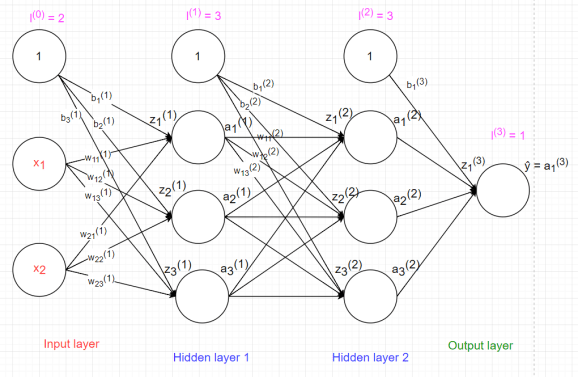
\includegraphics[scale=1]{chap2/c2_figs/nn_full-2.png}
\end{center}
\caption{Mô hình neural network trên gồm 3 layer. Input layer có 2 node $(l^{(0)} = 2$, hidden layer 1 có 3 node, hidden layer 2 có 3 node và output layer có 1 node.}
\label{fig:NN}
\end{figure}
\FloatBarrier

\textbf{Ký hiệu:}
\begin{itemize}
\item Số node trong hidden layer thứ $i$ là $l^{(i)}l(i)$.

\item Ma trận $W^{(k)}$ kích thước $l^{(k-1)}*l^{(k)}$ là ma trận hệ số giữa layer $(k-1)$ và layer $k$, trong đó $w_{ij}^{(k)}$ là hệ số kết nối từ node thứ $i$ của layer $k-1$ đến node thứ $j$ của layer $k$.

\item Vector $b^{(k)}$ kích thước $l^{k} * 1$ là hệ số bias của các node trong layer $k$, trong đó $b_i^{(k)}$ là bias của node thứ $i$ trong layer $k$. 
\end{itemize}

Với node thứ $i$ trong layer $l$ có bias $b_i^{(l)}$ thực hiện 2 bước:
\begin{itemize}
\item Tính tổng linear: $z_i^{(l)} = \sum_{j=1}^{l^{(l-1)}} a_j^{(l-1)} * w_{ji}^{(l)} + b_i^{(l)}$ là tổng tất cả các node trong layer trước nhân với hệ số w tương ứng, rồi cộng với bias b.
\item Áp dụng activation function: $a_i^{(l)} = \sigma(z_i^{(l)})$
\end{itemize}

Vector $z^{(k)}$ kích thước $l^{(k)} * 1$ là giá trị các node trong layer $k$ sau bước tính tổng linear.

Vector $a^{(k)}$ kích thước $l^{(k)} * 1$ là giá trị của các node trong layer $k$ sau khi áp dụng hàm activation function.



Do mỗi node trong hidden layer và output layer đều có bias nên trong input layer và hidden layer cần thêm node 1 để tính bias (nhưng không tính vào tổng số node layer có).

Tại node thứ 2 ở layer 1, ta có:

\begin{itemize}
\item $z_2^{(1)} =  x_1 * w_{12}^{(1)} +  x_2 * w_{22}^{(1)} + b_2^{(1)}$
\item $a_2^{(1)} = \sigma(z_2^{(1)})$
\end{itemize} 

Hay ở node thứ 3 layer 2, ta có:
\begin{itemize}
\item $z_3^{(2)} =  a_1^{(1)} * w_{13}^{(2)} + a_2^{(1)} * w_{23}^{(2)}  + a_3^{(1)} * w_{33}^{(2)} + b_3^{(2)}$
\item $a_2^{(1)} = \sigma(z_2^{(1)})$
\end{itemize} 

\subsection{Quá trình huấn luyện một mạng NN}

Quá trình huấn luyện một mạng NN được thể hiện qua sự lặp đi lặp lại hai bước sau:
\begin{itemize}
\item \textbf{Feedforward:} Lan truyền tiến. Dự đoán output $\hat{y}$ với một input $x$ bằng cách tính toán từ đầu đến cuối của mạng neuron.
\item \textbf{Backpropagation:} Lan truyền ngược và cập nhật trọng số.
\end{itemize}
\textbf{Bước 1: Lan truyền tiến}
Để nhất quán về mặt ký hiệu, gọi input layer là $a^{(0)} (=x)$ kích thước $2*1$.


\FloatBarrier
\begin{figure}[htp]
\begin{center}
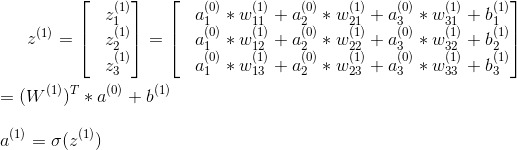
\includegraphics[scale=0.8]{chap2/c2_figs/feed_forward.jpg}
\end{center}
\label{fig:feed_forward0}
\end{figure}
\FloatBarrier
Tương tự ta có:
$\newline z^{(2)} = (W^{(2)})^T * a^{(1)} + b^{(2)}\newline  a^{(2)} = \sigma(z^{(2)}) \newline z^{(3)} = (W^{(3)})^T * a^{(2)} + b^{(3)}\newline  \hat{y} = a^{(3)} = \sigma(z^{(3)})$

\FloatBarrier
\begin{figure}[htp]
\begin{center}
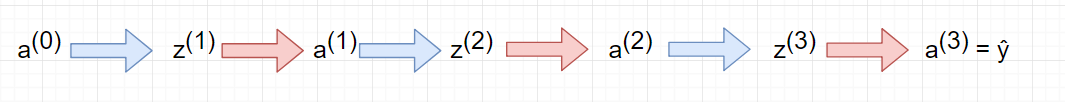
\includegraphics[scale=0.75]{chap2/c2_figs/ff.png}
\end{center}
\caption{Feedforward}
\label{fig:feed_forward}
\end{figure}
\FloatBarrier

\begin{itemize}
\item[$\square$] \textbf{Biểu diễn dưới dạng ma trận:}
\end{itemize}
Tuy nhiên khi làm việc với dữ liệu ta cần tính dự đoán cho nhiều dữ liệu một lúc, nên gọi $X$ là ma trận $n*d$, trong đó $n$ là số dữ liệu và $d$ là số trường trong mỗi dữ liệu, trong đó $x_j^{[i]}$ là giá trị trường dữ liệu thứ $j$ của dữ liệu thứ $i$.
Biểu diễn dạng ma trận của vector dữ liệu đầu vào như sau:

\FloatBarrier
\begin{figure}[htp]
\begin{center}
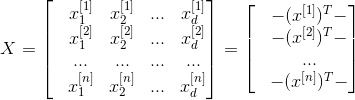
\includegraphics[scale=0.8]{chap2/c2_figs/1.jpg}
\end{center}
\label{fig:feed_forward}
\end{figure}
\FloatBarrier

Do $x^{[1]}$ là vector kích thước $d*1$ tuy nhiên ở $X$ mỗi dữ liệu được viết theo hàng nên cần transpose $x^{[1]}$ thành kích thước $1*d$, kí hiệu: $(x^{[1]})^T$
Gọi ma trận $Z^{(i)}$ kích thước$ N*l^{(i)}$ trong đó $z_{j}^{(i)[k]}$ là giá trị thứ $j$ trong layer $i$ sau bước tính tổng linear của dữ liệu thứ $k$ trong dataset.

*** Kí hiệu $(i)$ là layer thứ $i$ và kí hiệu $[k]$ là dữ liệu thứ $k$ trong dataset.

Tương tự, gọi ma trận $A^{(i)}$ kích thước $N*l^{(i)}$ trong đó $a_{j}^{(i)[k]}$ là giá trị thứ $j$ trong layer $i$ sau khi áp dụng activation function của dữ liệu thứ $k$ trong dataset.

\FloatBarrier
\begin{figure}[htp]
\begin{center}
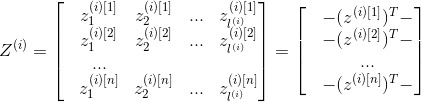
\includegraphics[scale=0.8]{chap2/c2_figs/2.jpg}
\end{center}
\label{fig:feed_forward}
\end{figure}
\FloatBarrier

Do đó:

\FloatBarrier
\begin{figure}[htp]
\begin{center}
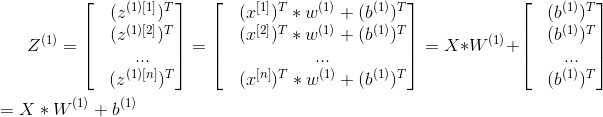
\includegraphics[scale=0.75]{chap2/c2_figs/3.jpg}
\end{center}
\label{fig:feed_forward}
\end{figure}
\FloatBarrier
Như vậy:

\FloatBarrier
\begin{figure}[htp]
\begin{center}
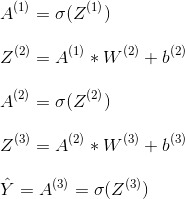
\includegraphics[scale=0.75]{chap2/c2_figs/4.jpg}
\end{center}
\label{fig:feed_forward}
\end{figure}
\FloatBarrier

Vậy là có thể tính được giá trị dự đoán của nhiều dữ liệu 1 lúc dưới dạng ma trận.

Giờ từ input $X$ ta có thể tính được giá trị dự đoán $\hat{Y}$, tuy nhiên việc chính cần làm là đi tìm hệ số $W$ và $b$. Có thể nghĩ ngay tới thuật toán gradient descent và việc quan trọng nhất trong thuật toán gradient descent là đi tìm đạo hàm của các hệ số đối với loss function. Và việc tính đạo hàm của các hệ số trong neural network được thực hiện bởi thuật toán backpropagation, sẽ được trình bày ở bước sau.

\textbf{Bước 2: Backpropagation - Lan truyền ngược và cập nhật trọng số}
Giờ ta cần đi tìm hệ số $W$ và $b$. Có thể nghĩ ngay tới thuật toán gradient descent và việc quan trọng nhất trong thuật toán gradient descent là đi tìm đạo hàm của các hệ số đối với loss function. Bước này sẽ tính đạo hàm của các hệ số trong neural network với thuật toán backpropagation.

Quá trình học vẫn là tìm lấy một hàm lỗi để đánh giá và tìm cách tối ưu hàm lỗi đó để được kết quả hợp lý nhất có thể. Với mỗi điểm $(x^{[i]}, y_i)$ ta có hàm loss function được tính theo công thức: $$L = -(y_i * log(\hat{y_i}) + (1 - y_i) * log(1 - \hat{y_i}))$$

Hàm loss function trên toàn bộ dữ liệu:
$$J = - \sum_{i=1}^{N}(y_i * log(\hat{y_i}) + (1 - y_i) * log(1 - \hat{y_i}))$$

\begin{itemize}
\item[$\blacksquare$] \textbf{Gradient Descent}
\end{itemize}
Để áp dụng gradient descent ta cần tính được đạo hàm của các hệ số W và bias b với hàm loss function.
*** Kí hiệu chuẩn về đạo hàm
\begin{itemize}
\item Khi hàm f(x) là hàm 1 biến x, ví dụ: $ f(x) = 2*x + 1$. Đạo hàm của $f$ đối với biến $x$ kí hiệu là $\frac{df}{dx}\newline $
\item Khi hàm $f(x, y)$ là hàm nhiều biến, ví dụ $ f(x, y) = x^2 + y^2$. Đạo hàm $f$ với biến $x$ kí hiệu là $ \frac{\partial f}{\partial x}$
\end{itemize}

Với mỗi điểm $(x^{([i]}, y_i)$, hàm loss function sẽ là:

$$L = -(y_i * log(\hat{y_i}) + (1 - y_i) * log(1 - \hat{y_i}))$$


trong đó: $\hat{y_i} = a_1^{(2)} = \sigma(a_1^{(1)} * w_{11}^{(2)} + a_2^{(1)} * w_{21}^{(2)} + b_1^{(2)})$
 là giá trị mà model dự đoán, còn $y_i$ là giá trị thật của dữ liệu.
$$\frac{\partial L}{\partial\hat{y_i}} = - \frac{\partial(y_i * log(\hat{y_i}) + (1 - y_i) * log(1 - \hat{y_i}))}{\partial\hat{y_i}}= - (\frac{y_i}{\hat{y_i}} - \frac{1-y_i}{(1-\hat{y})})\newline$$
Tính đạo hàm L với $W^{(2)}$, $b^{(2)}$\\
Áp dụng chain rule ta có: $$ \frac{\partial L}{\partial b_1^{(2)}} = \frac{dL}{d\hat{y_i}} * \frac{\partial\hat{y_i}}{\partial b_1^{(2)} } $$

\FloatBarrier
\begin{figure}[htp]
\begin{center}
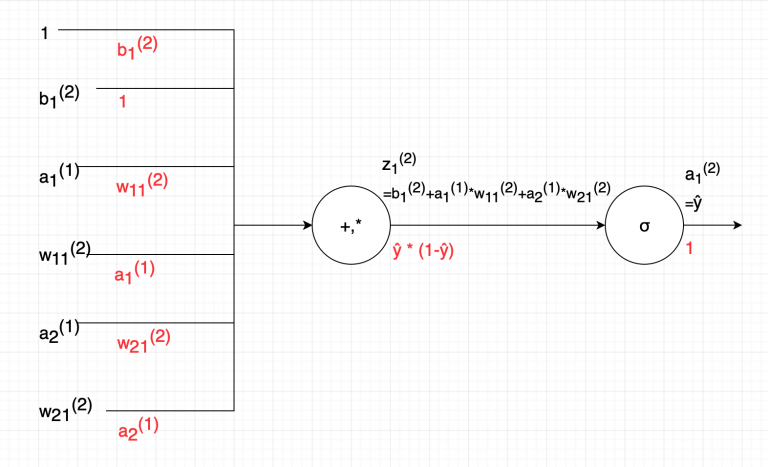
\includegraphics[scale=1]{chap2/c2_figs/6.png}
\end{center}
\label{fig:feed_forward}
\end{figure}
\FloatBarrier

Từ đồ thị ta thấy:

$$\frac{\partial\hat{y_i}}{\partial b_1^{(2)}} = \hat{y_i} * (1-\hat{y_i})\newline$$

$$\frac{\partial\hat{y_i}}{\partial w_{11}^{(2)}} = a_1^{(1)}*\hat{y_i} * (1-\hat{y_i})\newline$$

$$\frac{\partial\hat{y_i}}{\partial w_{21}^{(2)}} = a_2^{(1)}*\hat{y_i} * (1-\hat{y_i})\newline$$

$$\frac{\partial\hat{y_i}}{\partial a_1^{(1)} }=w_{11} ^{(2)}*\hat{y_i} * (1-\hat{y_i})\newline$$

$$\frac{\partial\hat{y_i}}{\partial a_2^{(1)} }=w_{21} ^{(2)}*\hat{y_i} * (1-\hat{y_i})\newline$$
Do đó:
$$\frac{\partial L}{\partial b_1^{(2)}} = \frac{\partial L}{\partial\hat{y_i}} * \frac {\partial\hat{y_i}}{\partial b_1^{(2)}} = - (\frac{y_i}{\hat{y_i}} - \frac{1-y_i}{(1-\hat{y_i})}) * \hat{y_i} * (1-\hat{y_i}) = -(y_i * (1-\hat{y_i}) - (1-y_i) * \hat{y_i})) = \hat{y_i}-y_i$$

Tương tự:
$$\frac{\partial L}{\partial w_{11} ^ {(2)}} = a_1 ^ {(1)} *     (\hat{y_i}-y_i)\newline \newline$$

$$\frac{\partial L}{\partial w_{21} ^ {(2)}} = a_2 ^ {(1)} *     (\hat{y_i}-y_i) \newline \newline$$

$$\frac{\partial L}{\partial a_1 ^ {(1)}} =  w_{11} ^ {(2)}  *     (\hat{y_i}-y_i) \newline \newline$$

$$\frac{\partial L}{\partial a_2 ^ {(1)}} =  w_{21} ^ {(2)}  *     (\hat{y_i}-y_i) \newline \newline $$


\begin{itemize}
\item[$\square$] \textbf{Biểu diễn dưới dạng ma trận:}
\end{itemize} 
\textbf{*** Lưu ý:} đạo hàm của L đối với ma trận W kích thước m*n cũng là một ma trận cùng kích thước $m*n$.

\FloatBarrier
\begin{figure}[htp]
\begin{center}
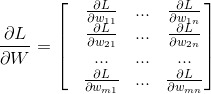
\includegraphics[scale=1]{chap2/c2_figs/5.jpg}
\end{center}
\label{fig:feed_forward}
\end{figure}
\FloatBarrier

Do đó:
$$\frac{\partial J}{\partial W^{(2)}} = (A^{(1)})^T * (\hat{Y} - Y), \frac{\partial J}{\partial b^{(2)}} = (sum(\hat{Y} - Y))^T,  \frac{\partial J}{\partial A^{(1)}} = (\hat{Y} - Y) * (W^{(2)})^T$$ 
là phép tính sum tính tổng các cột của ma trận.

\FloatBarrier
\begin{figure}[htp]
\begin{center}
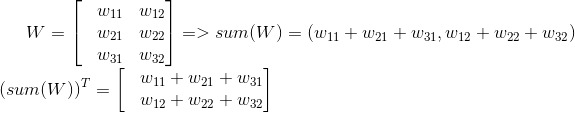
\includegraphics[scale=0.8]{chap2/c2_figs/6.jpg}
\end{center}
\label{fig:feed_forward}
\end{figure}
\FloatBarrier

Vậy là đã tính xong đạo hàm của $L$ với hệ số $W^{(2)}, b^{(2)}$. Giờ sẽ đi tính đạo hàm của $L$ với hệ số $W^{(1)}, b^{(1)}$ để khi tính đạo hàm của hệ số và bias trong layer trước đấy sẽ cần dùng đến.

Tính đạo hàm L với $W^{(1)}, b^{(1)}$
Do $ a_1^{(1)} = \sigma(b_1^{(1)} + x_1*w_{11}^{(1)} + x_2*w_{21}^{(1)})$ 

Áp dụng chain rule ta có: $$ \frac{\partial L}{\partial b_1^{(1)}} = \frac{\partial L}{\partial a_1^{(1)}} * \frac{\partial a_1^{(1)}}{\partial b_1^{(1)} }$$
Ta có:
$$\frac{\partial a_1^{(1)}}{\partial b_1^{(1)}} = \frac{\partial a_1^{(1)}}{z_1^{(1)}} * \frac{z_1^{(1)}}{\partial b_1^{(1)}} = a_1^{(1)} * (1 - a_1^{(1)})$$
Do đó:
$$\frac{\partial L}{\partial b_1^{(1)}} = a_1 ^ {(1)} * (1 - a_1^{(1)}) * w_{11}^{(2)} * (\hat{y_i} - y_i)$$

Tương tự:
$$\frac{\partial L}{\partial w_{11}^{(1)}} = x_1 * a_1 ^ {(1)} * (1 - a_1^{(1)}) * w_{11}^{(2)} *  (\hat{y_i} - y_i)  \newline$$

$$\frac{\partial L}{\partial w_{12}^{(1)}} = x_1 * a_2 ^ {(1)} * (1 - a_2^{(1)}) * w_{11}^{(2)} *  (\hat{y_i} - y_i)  \newline$$

$$\frac{\partial L}{\partial w_{21}^{(1)}} = x_2 * a_1 ^ {(1)} * (1 - a_1^{(1)}) * w_{21}^{(2)} *  (\hat{y_i} - y_i)  \newline $$

$$\frac{\partial L}{\partial w_{22}^{(1)}} = x_2 * a_2^ {(1)} * (1 - a_2^{(1)}) * w_{21}^{(2)} *  (\hat{y_i} - y_i)  \newline$$

Có thể tạm viết dưới dạng chain rule là: $$\frac{\partial J}{\partial W^{(1)}} = \frac{\partial J}{\partial A^{(1)}} * \frac{\partial A^{(1)}}{\partial Z^{(1)}}* \frac{\partial Z^{(1)}}{\partial W^{(1)}} (1) $$

Từ trên đã tính được: $$\frac{\partial J}{\partial A^{(1)}} = (\hat{Y} - Y) * (W^{(2)})^T$$

Đạo hàm của hàm sigmoid: $\frac{d\sigma(x)}{dx} = \sigma(x) * (1 - \sigma(x))$ và $A^{(1)} = \sigma(Z^{(1)})$ , nên trong (1) có thể hiểu là $\frac{\partial A^{(1)}}{\partial Z^{(1)}} = A^{(1)}* (1 - A^{(1)})$

Cuối cùng, $Z^{(1)} = X * W^{(1)} + b^{(1)}$ nên có thể tạm hiểu $\frac{\partial Z^{(1)}}{\partial W^{(1)}} = X$ , nó giống như $f(x)= a*x +b$ $ => \frac{df}{dx} = a$ .

Kết hợp tất cả lại ta được:
$$\frac{\partial J}{\partial W^{(1)}} = X^T * (((\hat{Y} – Y) * (W^{(2)})^T)\otimes A^{(1)}\otimes (1-A^{(1)}) ) $$

Vậy khi nào cần dùng element-wise $(\otimes)$, khi nào dùng nhân ma trận $(*)$?
\begin{itemize}
\item Khi tính đạo hàm ngược lại qua bước activation thì dùng $(\otimes)$.
\item Khi có phép tính nhân ma trận thì dùng $(*)$, nhưng đặc biệt chú ý đến \textbf{kích thước ma trận} và dùng \textbf{transpose} nếu cần thiết. Ví dụ: ma trận $X$ kích thước $N*3$, W kích thước $3*4$, $Z = X * W$ sẽ có kích thước $N*4$ thì $\frac{\partial J}{\partial W} = X^T * (\frac{\partial J}{\partial Z})$ và $\frac{\partial J}{\partial X} = (\frac{\partial J}{\partial Z}) * W^T$.
\end{itemize}
Tương tự: $$\frac{\partial L}{\partial b^{(1)}} = sum(((\hat{Y} – Y) * (W^{(2)})^T)\otimes A^{(1)})^T$$

Vậy là đã tính xong hết đạo hàm của loss function với các hệ số $W$ và bias $b$, giờ có thể áp dụng gradient descent để giải bài toán.

Giờ thử tính $ \frac{\partial L}{\partial x_1}$, ở bài này thì không cần vì chỉ có 1 hidden layer, nhưng nếu nhiều hơn 1 hidden layer thì cần phải tính bước này để tính đạo hàm với các hệ số trước đó.

\FloatBarrier
\begin{figure}[htp]
\begin{center}
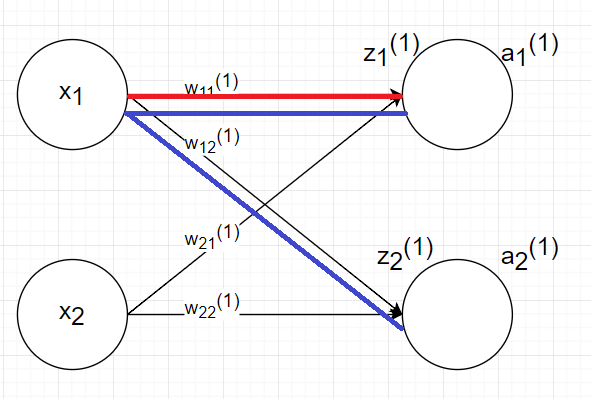
\includegraphics[scale=0.75]{chap2/c2_figs/1.png}
\end{center}
\caption{Đường màu đỏ cho $w_{11}^{(1)}$, đường màu xanh cho $x_1$}
\label{fig:feed_forward}
\end{figure}
\FloatBarrier

Ta thấy $w_{11}^{(1)}$ chỉ tác động đến $a_1^{(1)}$, cụ thể là $ a_1^{(1)} = \sigma(b_1^{(1)} + x_1*w_{11}^{(1)} + x_2*w_{21}^{(1)})$ 

Tuy nhiên $x_1$ không những tác động đến $a_1^{(1)}$ mà còn tác động đến $a_2^{(1)}$, nên khi áp dụng chain rule tính đạo hàm của $L$ với $x_1$ cần tính tổng đạo hàm qua cả $a_1^{(1)}$ và $a_2^{(1)}$.

\FloatBarrier
\begin{figure}[htp]
\begin{center}
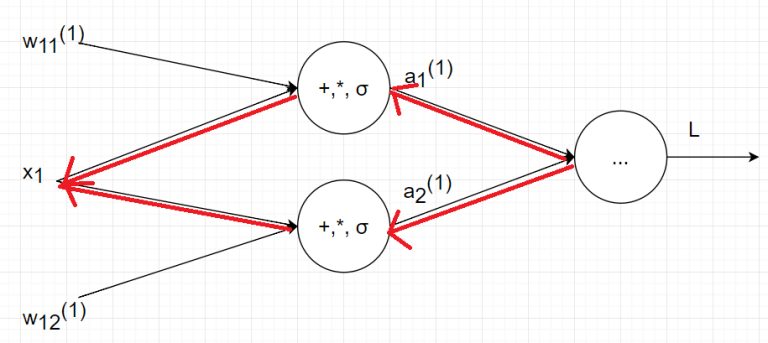
\includegraphics[scale=0.75]{chap2/c2_figs/2.png}
\end{center}
\caption{backpropagation tác động trong lớp ẩn}
\label{fig:feed_forward}
\end{figure}
\FloatBarrier

Do đó:
$$\frac{\partial L}{\partial x_1} = \frac{\partial L}{\partial a_1^{(1)}} * \frac{\partial a_1^{(1)}}{\partial x_1} + \frac{\partial L}{\partial a_2^{(1)}} * \frac{\partial a_2^{(1)}}{\partial x_1} =  w_{11}^{(1)}* a_1 ^ {(1)} * (1 – a_1^{(1)}) * w_{11}^{(2)} * (y_i – \hat{y_i}) + w_{12}^{(1)}* a_2 ^ {(1)} * (1 – a_2^{(1)}) * w_{21}^{(2)} * (y_i – \hat{y_i})  \newline$$

Sau tất cả, mô hình tổng quát sẽ bao gồm các bước như sau:

\FloatBarrier
\begin{figure}[htp]
\begin{center}
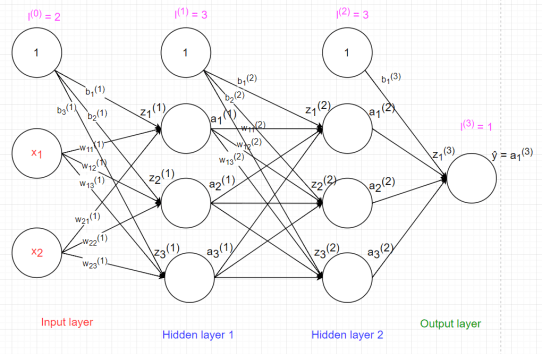
\includegraphics[scale=0.75]{chap2/c2_figs/3.png}
\end{center}
\caption{Mô hình neural network}
\label{fig:feed_forward}
\end{figure}
\FloatBarrier

\begin{itemize}
\item \textbf{Bước 1:} Tính $\frac{\partial J}{\partial \hat{Y}}$, trong đó $\hat{Y} = A^{(3)}$
\item \textbf{Bước 2:} Tính $$\frac{\partial J}{\partial \hat{W^{(3)}}}= (A^{(2)})^T * (\frac{\partial J}{\partial \hat{Y}} \otimes \frac{\partial A^{(3)}}{\partial Z^{(3)}}),  \frac{\partial J}{\partial \hat{b^{(3)}}}= (sum( \frac{\partial J}{\partial \hat{Y}} \otimes \frac{\partial A^{(3)}}{\partial Z^{(3)}}))^T$$
\item \textbf{Bước 3:} Tính $$\frac{\partial J}{\partial \hat{W^{(2)}}}= (A^{(1)})^T * (\frac{\partial J}{\partial A^{(2)}} \otimes \frac{\partial A^{(2)}}{\partial Z^{(2)}}),  \frac{\partial J}{\partial \hat{b^{(2)}}}= (sum (\frac{\partial J}{\partial A^{(2)}} \otimes \frac{\partial A^{(2)}}{\partial Z^{(2)}}))^T$$ và tính $$\frac{\partial J}{\partial \hat{A^{(1)}}}= ( \frac {\partial J}{\partial A^{(2)}} \otimes \frac{\partial A^{(2)}}{\partial Z^{(2)}}) * (W^{(2)})^T$$ 
\item \textbf{Bước 4:} Tính $$\frac{\partial J}{\partial \hat{W^{(1)}}}= (A^{(0)})^T  * (\frac{\partial J}{\partial A^{(1)}} \otimes \frac{\partial A^{(1)}}{\partial Z^{(1)}}),  \frac{\partial J}{\partial \hat{b^{(1)}}}= (sum (\frac{\partial J}{\partial A^{(1)}} \otimes \frac{\partial A^{(1)}}{\partial Z^{(1)}}))^T$$ , trong đó $A^{(0)} = X$
\end{itemize}

Nếu network có nhiều layer hơn thì cứ tiếp tục cho đến khi tính được đạo hàm của loss function $J$ với tất cả các hệ số $W$ và bias $b$.

Nếu hàm activation là sigmoid thì $\frac{\partial A^{(i)}}{\partial Z^{(i)}} = A^{(i)} \otimes (1-A^{(i)})$

Tổng kết lại, 2 quá trình Feedfoward và Backpropagation sẽ diễn ra lần lượt như sau:

\FloatBarrier
\begin{figure}[htp]
\begin{center}
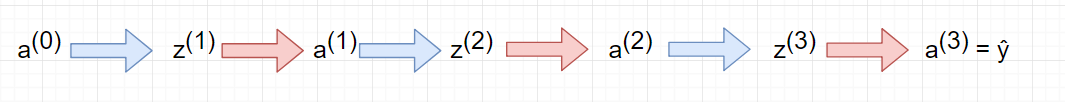
\includegraphics[scale=0.7]{chap2/c2_figs/7.png}
\end{center}
\end{figure}
\FloatBarrier

\FloatBarrier
\begin{figure}[htp]
\begin{center}
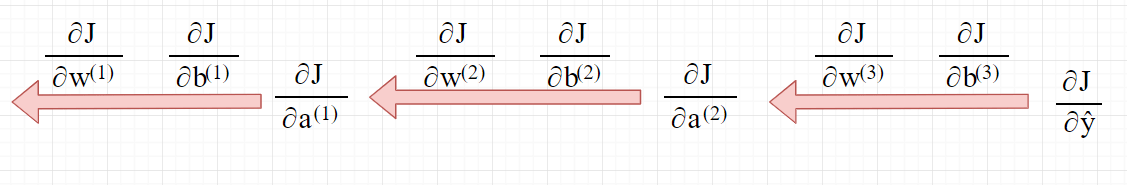
\includegraphics[scale=0.65]{chap2/c2_figs/8.png}
\end{center}
\caption{Feedforward và Backpropagation}
\label{fig:backpropagation}
\end{figure}
\FloatBarrier

(Theo "Sách Deep Learning cơ bản" - tác giả: Nguyễn Thanh Tuấn)

\section{Mạng Convolutional Neural Network (CNN)}
Convolutional Neural Network (CNNs – Mạng nơ-ron tích chập) là một trong những mô hình Deep Learning tiên tiến giúp cho chúng ta xây dựng được những hệ thống thông minh với độ chính xác cao như hiện nay. Trong luận văn này, sẽ trình bày về Convolution (tích chập) đi từ những khái niệm cơ bản nhất đến ứng dụng của nó cũng như ý tưởng của mô hình CNNs trong phát hiện và trích xuất đặc trưng khung xương từ ảnh RGB.

Mạng Neural Network truyền thống tuy đã giải quyết  được một số vấn đề lớn lúc bấy giờ nhưng lại gặp một số khó khăn khi giải quyết bài toán xử lý, phân loại hình ảnh.
Đối với mạng Neural Network truyền thống khi xử lý ảnh màu 64*64 được biểu diễn dưới dạng 1 tensor 64*64*3. Việc để biểu thị hết nội dung của bức ảnh thì cần truyền vào input layer tất cả các pixel (64*64*3 = 12288). Nghĩa là input layer giờ có 12288 nodes. Giả sử số lượng node trong hidden layer 1 là 1000. Số lượng weight $W$ giữa input layer và hidden layer 1 là 12288*1000 = 12288000, số lượng bias là 1000 $=>$ tổng số parameter là: 12289000. Đây mới chỉ là số parameter giữa input layer và hidden layer 1, trong model còn nhiều layer nữa, và nếu kích thướcây ảnh tăng, ví dụ 512*512 thì số lượng parameter tăng cực kì nhanh. Điều này khiến cho việc tính toán của máy tính cần rất nhiều công sức nhưng lại không mang lại hiệu quả cao. Do vậy ta cần có giải pháp tốt hơn.

Nhận xét:
\begin{itemize}
\item Trong ảnh các pixel ở cạnh nhau thường có liên kết với nhau hơn là những pixel ở xa. Ví dụ để thể hiện một vật thể trên ảnh cần các pixel gần nhau và có màu sắc tương tự nhau.
\item Ngoài ra để so sánh các đối tượng là giống hay khác nhau cần phải so sánh giữa khu vực này với khu vực kia của bức ảnh. Do vậy cần phải có một bộ hệ số tính toán với các pixel quét hết toàn bộ bức ảnh để so sánh các vùng. Hay nói cách khác là các pixel ảnh chia sẻ hệ số với nhau.
\end{itemize}
=> Do vậy ý tưởng sử dụng mạng Convolutional Neural Network ra đời. Áp dụng phép tính convolution vào layer trong neural network ta có thể giải quyết được vấn đề lượng lớn parameter mà vẫn lấy ra được các đặc trưng của ảnh.
\subsection{Phép Tính Convolution}
\label{ss: convolution}
Để cho dễ hình dung mình sẽ lấy ví dụ trên ảnh xám, tức là ảnh được biểu diễn dưới dạng ma trận $A$ kích thước $m*n$.
Ta định nghĩa kernel là một ma trận vuông kích thước $k*k$ trong đó $k$ là số lẻ. $k$ có thể bằng $1, 3, 5, 7, 9,…$ Ví dụ kernel kích thước $3*3$.

Kí hiệu phép tính convolution $(\otimes)$, kí hiệu $Y = X \otimes W$.

Với mỗi phần tử $x_{ij}$ trong ma trận $X$ lấy ra một ma trận có kích thước bằng kích thước của kernel $W$ có phần tử $x_{ij}$ làm trung tâm (đây là vì sao kích thước của kernel thường lẻ) gọi là ma trận $A$. Sau đó tính tổng các phần tử của phép tính element-wise của ma trận $A$ và ma trận $W$, rồi viết vào ma trận kết quả $Y$.

\FloatBarrier
\begin{figure}[htp]
\begin{center}
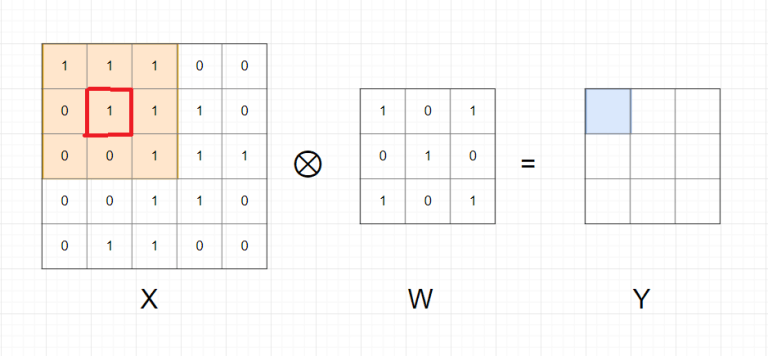
\includegraphics[scale=0.65]{chap2/c2_figs/9.png}
\end{center}
\caption{Phép tính Convolution}
\label{fig:convolution}
\end{figure}
\FloatBarrier

Ví dụ khi tính tại $x_{22}$ (ô khoanh đỏ trong hình \ref{fig:convolution}), ma trận $A$ cùng kích thước với $W$, có $x_{22}$ làm trung tâm có màu nền da cam như trong hình. Sau đó tính $y_{11} = sum(A \otimes W) = x_{11}*w_{11} + x_{12}*w_{12} + x_{13}*w_{13} + x_{21}*w_{21} + x_{22}*w_{22} + x_{23}*w_{23} + x_{31}*w_{31} + x_{32}*w_{32} + x_{33}*w_{33} = 4$. Và làm tương tự với các phần tử còn lại trong ma trận.

Vì tâm của kernel $W$ không thể lướt hết ma trận $X$ nên $Y$ sẽ có kích thước nhỏ hơn ma trận $X$. Kích thước của ma trận Y là (m-k+1) * (n-k+1).

\FloatBarrier
\begin{figure}[htp]
\begin{center}
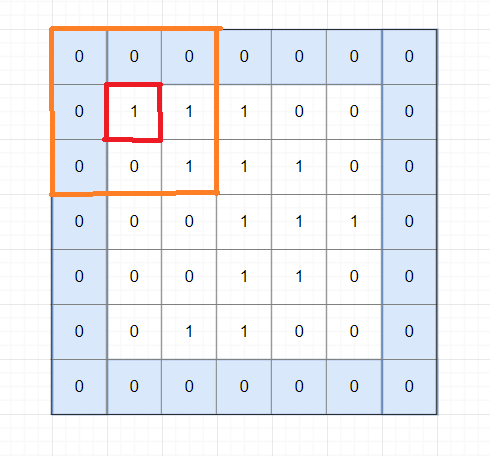
\includegraphics[scale=0.65]{chap2/c2_figs/10.png}
\end{center}
\caption{Convolution feature có kích thước nhỏ hơn ảnh ban đầu}
\label{fig:convolution-feature}
\end{figure}
\FloatBarrier

\begin{itemize}
\item[$\blacksquare$] \textbf{Padding}
Mỗi lần thực hiện phép tính convolution xong thì kích thước ma trận Y đều nhỏ hơn X. Tuy nhiên giờ ta muốn ma trận Y thu được có kích thước bằng ma trận X vì vậy cần tìm cách giải quyết cho các phần tử ở viền bằng cách thêm giá trị 0 ở viền ngoài ma trận X.

\FloatBarrier
\begin{figure}[htp]
\begin{center}
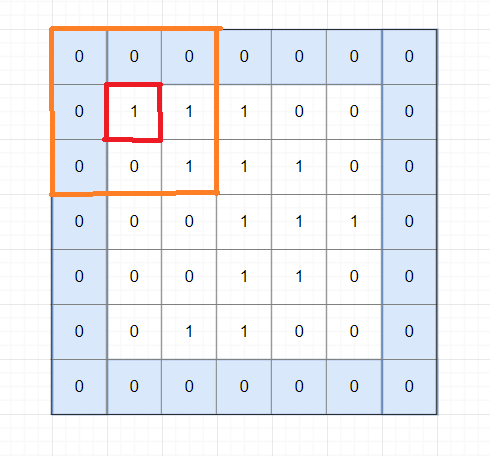
\includegraphics[scale=0.65]{chap2/c2_figs/10.png}
\end{center}
\caption{Ma trận X có viền 0 bên ngoài}
\label{fig:padding}
\end{figure}
\FloatBarrier

Rõ ràng là giờ đã giải quyết được vấn đề tìm A cho phần tử $x_{11}$, và ma trận $Y$ thu được sẽ bằng kích thước ma trận $X$ ban đầu.

Phép tính này gọi là convolution với $padding=1$. $Padding=k$ nghĩa là thêm $k$ vector $0$ vào mỗi phía của ma trận.

\item[$\blacksquare$] \textbf{Stride}
Như ở trên ta thực hiện tuần tự các phần tử trong ma trận $X$, thu được ma trận $Y$ cùng kích thước ma trận $X$, ta gọi là $stride=1$.

\FloatBarrier
\begin{figure}[htp]
\begin{center}
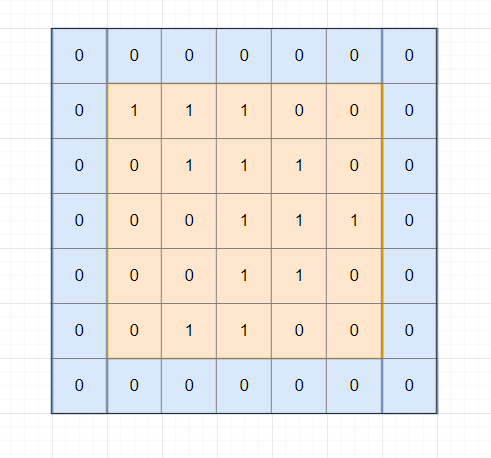
\includegraphics[scale=0.65]{chap2/c2_figs/11.png}
\end{center}
\caption{$stride=1, padding=1$}
\label{fig:padding}
\end{figure}
\FloatBarrier

Tuy nhiên nếu $stride=k (k > 1)$ thì ta chỉ thực hiện phép tính convolution trên các phần tử $x_{1+i*k,1+j*k}$. Ví dụ $k = 2$.

\FloatBarrier
\begin{figure}[htp]
\begin{center}
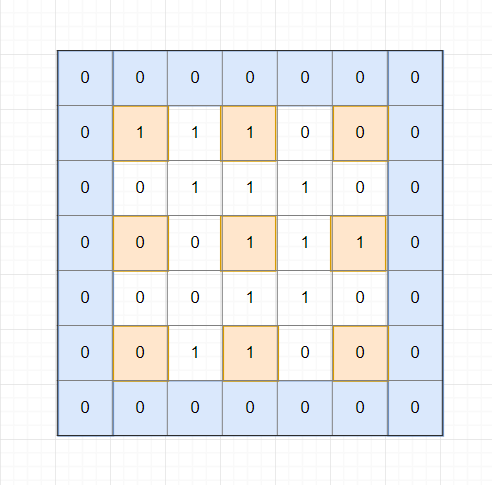
\includegraphics[scale=0.65]{chap2/c2_figs/12.png}
\end{center}
\caption{$padding=1, stride=2$}
\label{fig:padding,stride}
\end{figure}
\FloatBarrier

Hiểu đơn giản là bắt đầu từ vị trí $x_{11}$ sau đó nhảy $k$ bước theo chiều dọc và ngang cho đến hết ma trận $X$.

Kích thước của ma trận $Y$ là $3*3$ đã giảm đi đáng kể so với ma trận $X$.
Công thức tổng quát cho phép tính convolution của ma trận $X$ kích thước $m*n$ với kernel kích thước $k*k$, $stride = s$, $padding = p$ ra ma trận $Y$ kích thước $$(\frac{m-k+2p}{s}+1) * (\frac{n-k+2p}{s}+1)$$
Stride thường dùng để giảm kích thước của ma trận sau phép tính convolution.
Ý nghĩa của phép tính convolution:
Mục đích của phép tính convolution trên ảnh là làm mở, làm nét ảnh; xác định các đường;… Mỗi kernel khác nhau thì sẽ phép tính convolution sẽ có ý nghĩa khác nhau. 
\end{itemize} 
\subsection{Phép convolution trong mạng Neuron Network}
Với ảnh màu có tới 3 channels red, green, blue nên khi biểu diễn ảnh sẽ dưới dạng tensor 3 chiều. Nên ta cũng sẽ định nghĩa kernel là 1 tensor 3 chiều kích thước $k*k*3$.

\FloatBarrier
\begin{figure}[htp]
\begin{center}
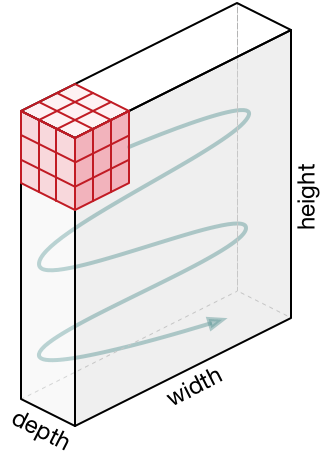
\includegraphics[scale=0.5]{chap2/c2_figs/13.png}
\end{center}
\caption{Phép tính convolution trên ảnh màu với k=3.}
\label{fig:padding,stride}
\end{figure}
\FloatBarrier

Ta định nghĩa kernel có cùng độ sâu (depth) với biểu diễn ảnh, rồi sau đó thực hiện di chuyển khối kernel tương tự như khi thực hiện trên ảnh xám.

\FloatBarrier
\begin{figure}[htp]
\begin{center}
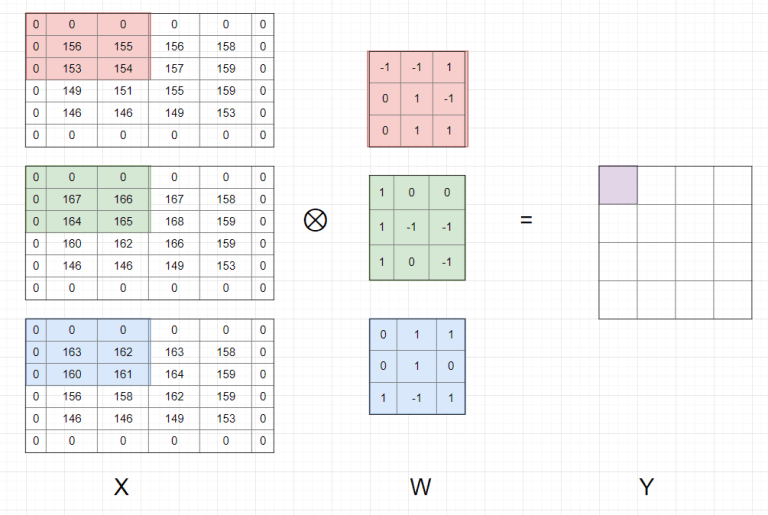
\includegraphics[scale=1]{chap2/c2_figs/14.png}
\end{center}
\caption{Tensor $X$ và $W$ 3 chiều được viết dưới dạng 3 matrix.}
\label{fig:padding,stride}
\end{figure}
\FloatBarrier

Khi biểu diễn ma trận ta cần 2 chỉ số hàng và cột: $i$ và $j$, thì khi biểu diễn ở dạng tensor 3 chiều cần thêm chỉ số độ sâu $k$. Nên chỉ số mỗi phần tử trong tensor là $x_{ijk}$.
$$y_{11} = b + (x_{111}*w_{111} +  x_{121}*w_{121} + x_{131}*w_{131} +  x_{211}*w_{211} +  x_{221}*w_{221} +  x_{231}*w_{231} +  x_{311}*w_{311} + $$ $$ x_{321}*w_{321} +  x_{331}*w_{331}) + (x_{112}*w_{112} +  x_{122}*w_{122} + x_{132}*w_{132} +  x_{212}*w_{212} +  x_{222}*w_{222} + $$ $$x_{232}*w_{232} +  x_{312}*w_{312} +  x_{322}*w_{322} +  x_{332}*w_{332}) +  (x_{113}*w_{113} +  x_{123}*w_{123} + x_{133}*w_{133} +  x_{213}*w_{213} + $$ $$ x_{223}*w_{223} +  x_{233}*w_{233} +  x_{313}*w_{313} +  x_{323}*w_{323} +  x_{333}*w_{333}) = -25$$

\FloatBarrier
\begin{figure}[htp]
\begin{center}
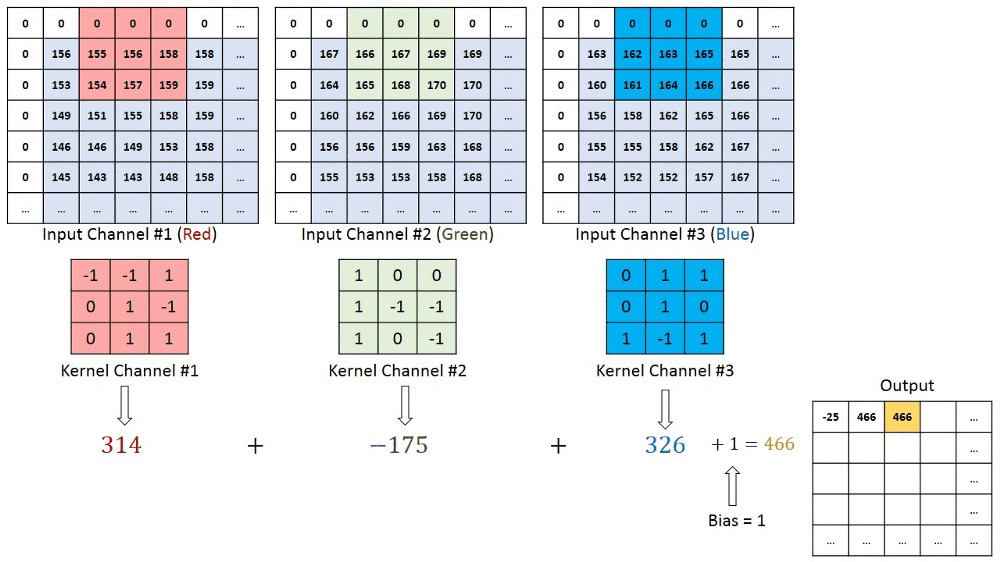
\includegraphics[scale=0.456]{chap2/c2_figs/8.jpg}
\end{center}
\caption{Thực hiện phép tính convolution trên ảnh màu}
\label{fig:padding,stride}
\end{figure}
\FloatBarrier

Nhận xét:
\begin{itemize}
\item Output Y của phép tính convolution trên ảnh màu là 1 matrix.
\item Có 1 hệ số bias được cộng vào sau bước tính tổng các phần tử của phép tính element-wise.
\end{itemize}

Với mỗi kernel khác nhau ta sẽ học được những đặc trưng khác nhau của ảnh, nên trong mỗi convolutional layer ta sẽ dùng nhiều kernel để học được nhiều thuộc tính của ảnh. Vì mỗi kernel cho ra output là 1 matrix nên k kernel sẽ cho ra k output matrix. Ta kết hợp k output matrix này lại thành 1 tensor 3 chiều có chiều sâu k.

\FloatBarrier
\begin{figure}[htp]
\begin{center}
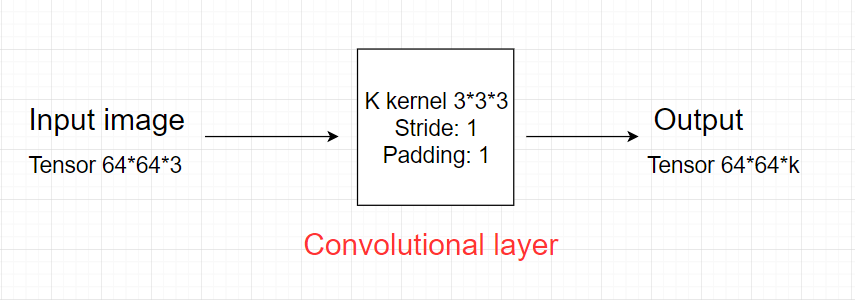
\includegraphics[scale=0.8]{chap2/c2_figs/15.png}
\end{center}
\caption{Convolutional layer đầu tiên}
\label{fig:conv-firstlayer}
\end{figure}
\FloatBarrier

Output của convolutional layer đầu tiên sẽ thành input của convolutional layer tiếp theo.

Convolutional layer tổng quát
Giả sử input của 1 convolutional layer tổng quát là tensor kích thước $H * W * D$.

Kernel có kích thước $F * F * D$ (kernel luôn có depth bằng depth của input và $F$ là số lẻ), stride: $S$, padding: $P$.

Convolutional layer áp dụng $K$ kernel.
=> Output của layer là tensor 3 chiều có kích thước: $ (\frac{H-F+2P}{S} + 1) * (\frac{W-F+2P}{S} + 1) * K$

\FloatBarrier
\begin{figure}[htp]
\begin{center}
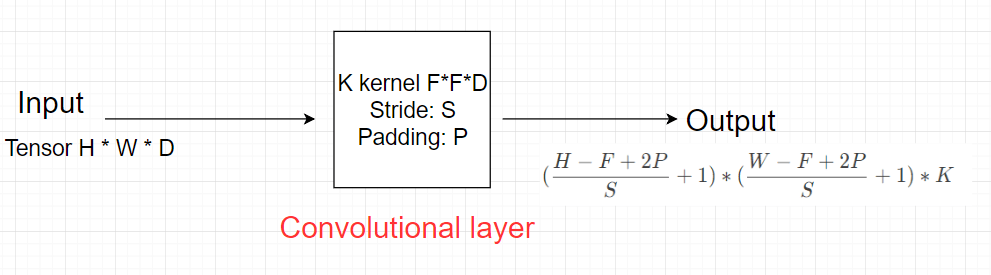
\includegraphics[scale=0.8]{chap2/c2_figs/16.png}
\end{center}
\caption{Convolutional layer tổng quát}
\label{fig:conv-tongquat}
\end{figure}
\FloatBarrier

Lưu ý:
\begin{itemize}
\item Output của convolutional layer sẽ qua hàm activation function trước khi trở thành input của convolutional layer tiếp theo.
\item Tổng số parameter của layer: Mỗi kernel có kích thước $F*F*D$ và có 1 hệ số bias, nên tổng parameter của 1 kernel là $F*F*D + 1$. Mà convolutional layer áp dụng $K$ kernel => Tổng số parameter trong layer này là $K * (F*F*D + 1)$.
\end{itemize}
Mạng Convolution Neural Network, ngoài các lớp Convolution ra còn có các lớp Pooling, Dropout, Dense, và Backnomalization,... để làm cho chúng trở nên "dễ học" hơn.


\subsection{Pooling layer}
\label{ss:Pooling}
Pooling layer thường được dùng giữa các convolutional layer, để giảm kích thước dữ liệu nhưng vẫn giữ được các thuộc tính quan trọng. Kích thước dữ liệu giảm giúp giảm việc tính toán trong model.

Gọi pooling size kích thước $K*K$. Input của pooling layer có kích thước $H*W*D$, ta tách ra làm $D$ ma trận kích thước $H*W$. Với mỗi ma trận, trên vùng kích thước $K*K$ trên ma trận ta tìm maximum hoặc average của dữ liệu rồi viết vào ma trận kết quả. Quy tắc về stride và padding áp dụng như phép tính convolution trên ảnh.

\FloatBarrier
\begin{figure}[htp]
\begin{center}
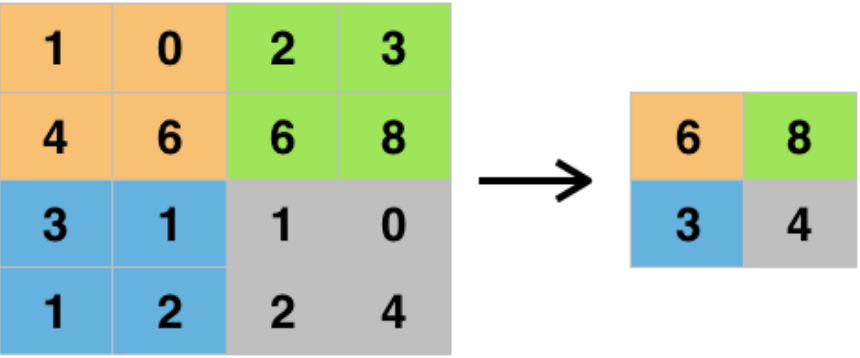
\includegraphics[scale=0.3]{chap2/c2_figs/9.jpg}
\end{center}
\caption{Phép Pooling với $stride=2, padding=0$}
\label{fig:pooling}
\end{figure}
\FloatBarrier

Nhưng hầu hết khi dùng pooling layer thì sẽ dùng $size=(2,2)$, $stride=2$, $padding=0$. Khi đó output width và height của dữ liệu giảm đi một nửa, depth thì được giữ nguyên.

\FloatBarrier
\begin{figure}[htp]
\begin{center}
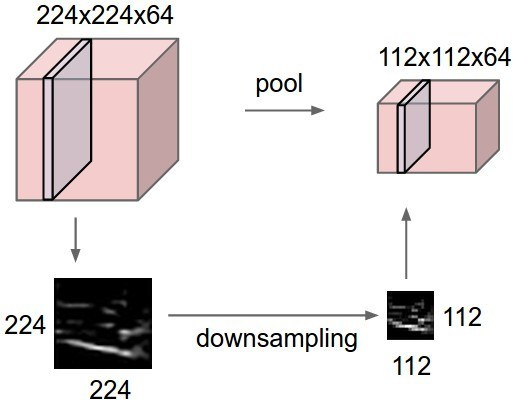
\includegraphics[scale=0.5]{chap2/c2_figs/pooling.jpeg}
\end{center}
\caption{Kết quả sau khi qua pooling layer $2*2$.}
\label{fig:pooling}
\end{figure}
\FloatBarrier
\centerline{http://cs231n.github.io/convolutional-networks/}

Có 2 loại pooling layer phổ biến là: max pooling và average pooling.
\FloatBarrier
\begin{figure}[htp]
\begin{center}
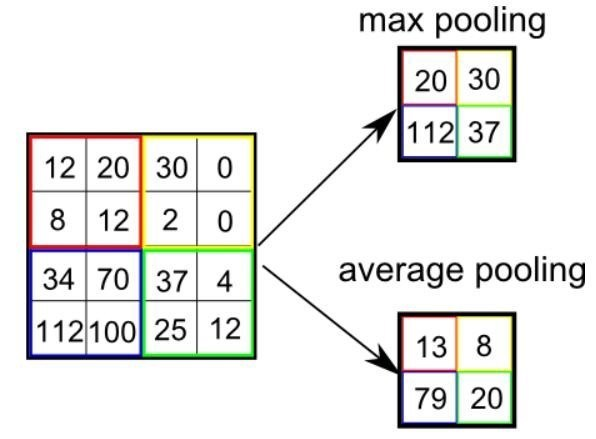
\includegraphics[scale=0.5]{chap2/c2_figs/10.jpg}
\end{center}
\caption{Max pooling và average pooling}
\label{fig:pooling}
\end{figure}
\FloatBarrier
Ngoài ra còn có thể dùng convolutional layer với stride > 1 để giảm kích thước dữ liệu thay cho pooling layer.

\subsection{Fully connected layer (Dense layer)}
\label{ss:dense}
Sau khi ảnh được truyền qua nhiều convolutional layer và pooling layer thì model đã học được tương đối các đặc điểm của ảnh (ví dụ mắt, mũi, khung mặt,…) thì tensor của output của layer cuối cùng, kích thước $H*W*D$, sẽ được chuyển về 1 vector kích thước $(H*W*D)$.

\FloatBarrier
\begin{figure}[htp]
\begin{center}
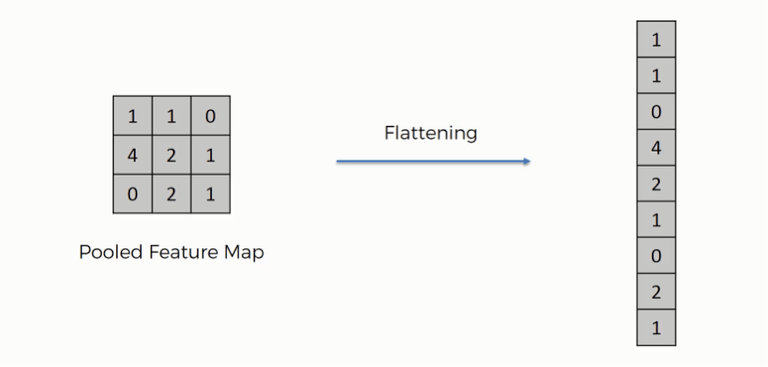
\includegraphics[scale=1]{chap2/c2_figs/17.png}
\end{center}
\caption{Phép Flatten biến tensor về 1 vector}
\label{fig:flatten}
\end{figure}
\FloatBarrier
Sau đó, mỗi điểm của vector sẽ được liên kết với toàn bộ output của mode giống như 1 lớp của mạng Neural Network truyền thống.Và cuối cùng của mạng sẽ có nhiệm vụ phân loại theo như yêu cầu của từng bài toán. Thường sẽ sử dụng hàm softmax để tính đầu ra cho lớp này.




\subsection{Kết luận}
Tổng hợp lại, một mô hình mạng CNN sẽ có cấu trúc chung gần giống như hình \ref{fig:tonghopCNN}

\FloatBarrier
\begin{figure}[htp]
\begin{center}
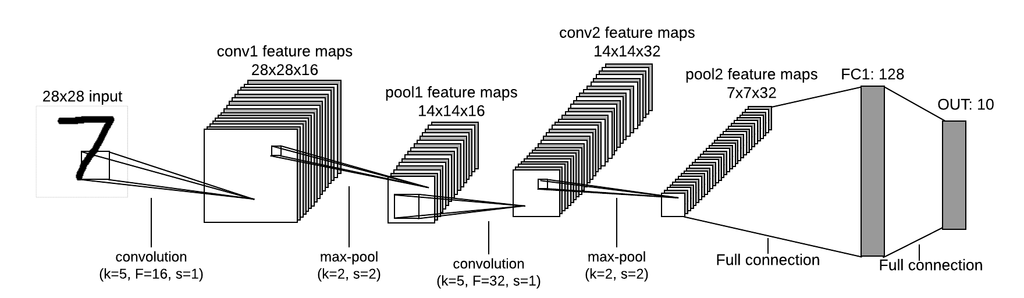
\includegraphics[scale=1]{chap2/c2_figs/18.png}
\end{center}
\caption{Ví dụ mô hình 1 môn hình convolutional neural network}
\label{fig:flatten}
\end{figure}
\FloatBarrier
\centerline{Input image -> Convolutional layer (Conv) + Pooling layer (Pool) -> Fully connected layer (FC) -> Output}
\centerline{Nguồn: https://www.easy-tensorflow.com/tf-tutorials/convolutional-neural-nets-cnns}

\newpage
\chapter{ƯỚC TÍNH TỌA ĐỘ KHUNG XƯƠNG TỪ ẢNH RGB}
\label{s:pose estimate}
Trong nội dung này, em sẽ trình bày hai phương pháp đề xuất để trích xuất đặc trưng khung xương. Đó là trích xuất đặc trưng từ thiết bị Kinect và trích xuất đặc trưng từ mạng neuron network. Phương pháp trích xuất đặc trưng khung xương từ ảnh RGB qua mạng NN dựa trên mạng mobilenet v2 được áp dụng trong đề tài vì tính khả thi, có thể ứng dụng được trong đời sống cao hơn so với phương pháp sử dụng camera Kinect.

\section{ƯỚC TÍNH DỰA TRÊN CAMERA ĐỘ SÂU KINECT}
\label{ss:kinect}
\subsection{Giới thiệu camera cảm biến độ sâu Kinect của Microsoft}
Kinect là một thiết bị đầu vào,là cảm biến chuyển động do hãng Microsoft sản xuất dành cho Xbox 360 và máy tính Windows. Dựa trên một webcam kiểu add-on ngoại vi cho Xbox 360, nó cho phép người dùng điều khiển và tương tác với Xbox 360 mà không cần phải dùng đến một bộ điều khiển tay cầm, thông qua một giao diện người dùng tự nhiên bằng cử chỉ và lệnh nói. Thiết bị được giới thiệu vào tháng 11 năm 2010 như một phụ kiện của Xbox 360. Cảm biến chiều sâu (depth sensor) được sử dụng trong Kinect được lấy từ việc trích xuất camera hồng ngoại. 

Chức năng chính của Kinect là một công cụ để người dùng tương tác với Xbox 360 bằng cử chỉ và lệnh nói. Vì lý do này, các bộ cảm biến có khả năng thu thập dữ liệu ở độ phân giải 640x480 điểm ảnh. Với các dữ liệu chiều sâu, có thể lấy được "các vector đặc trưng mang hình dáng của khung xương con người(SJMs)" của người đứng phía trước của cảm biến. Và với các SJM đó, nó có thể nhận biết được cử chỉ của người sử dụng.

\FloatBarrier
\begin{figure}[htp]
\begin{center}
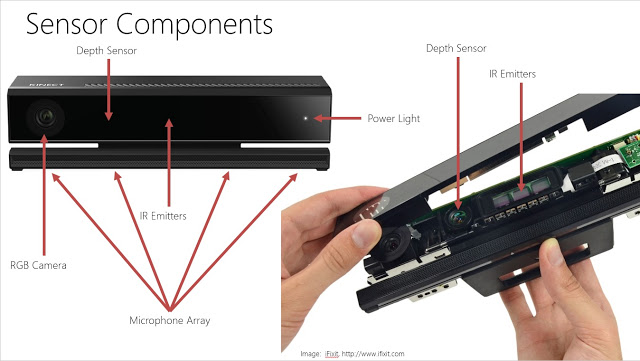
\includegraphics[scale=0.8]{chap3/c3_figs/kinect.png}
\end{center}
\caption{Camera cảm biến độ sâu Kinect \\(Nguồn : \url{https://www.ifixit.com)}}
\label{fig:kinect}
\end{figure}
\FloatBarrier

Các thông số cơ bản của cảm biến như sau:
\begin{itemize}
\item Ảnh màu : 1920x1080 @30Hz (15Hz ánh sáng yếu)
\item Ảnh độ sâu : 512x424 @30Hz
\item Tầm xa : 0.5 $\sim$ 4.5m
\item Góc nhìn (Dọc/Ngang) : 70 / 60 độ
\item Số lượng SJM (phát hiện/theo dõi) : 6 / 6 SJMs
\item Số lượng SJM-J : 25 SJM-Js
\item Hệ điều hành : Windows 8/10
\item Cổng tín hiệu : USB 3.0
\end{itemize}

Cơ chế hoạt động: Ban đầu, bộ phần phát tia hồng ngoại sẽ phát ra tia hồng ngoại trong vùng hoạt động của nó. Thông qua phản chiếu các tia hồng ngoại về camera hồng ngoại sẽ thu nhận được các tia phản xạ về. Dựa vào thời gian trễ để đo khoảng cách tới các điểm trong vùng quan sát. Kết quả thu về sẽ là hình ảnh vùng quan sát với những chiều sâu khác nhau.

\FloatBarrier
\begin{figure}[htp]
\begin{center}
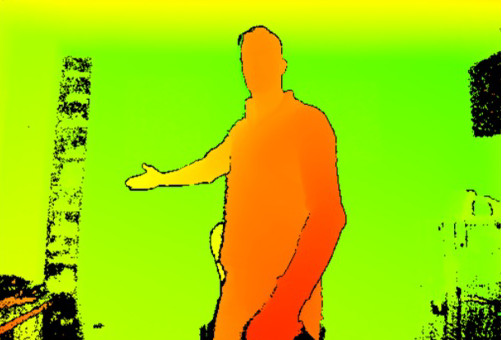
\includegraphics[scale=0.8]{chap3/c3_figs/depth.jpg}
\end{center}
\caption{Ảnh độ sâu từ Kinect \\(Nguồn : \url{https://www.zonetrigger.com/)}}
\label{fig:kinect}
\end{figure}
\FloatBarrier

\subsection{Cơ chế trích xuất SJM từ Kinect}
Ưu điểm của việc sử dụng Kinect là các thiết kế phần cứng đã tối ưu cho việc tạo ra SJM, không yêu cầu phải thực hiện lại hoặc tạo ra thuật toán mới cho phần trích xuất đặc trưng. Sơ đồ khối trích xuất SJM của Kinect v2 minh họa bằng hình \ref{fig:TrichKhungXuong}.

\FloatBarrier
\begin{figure}[htp]
\begin{center}
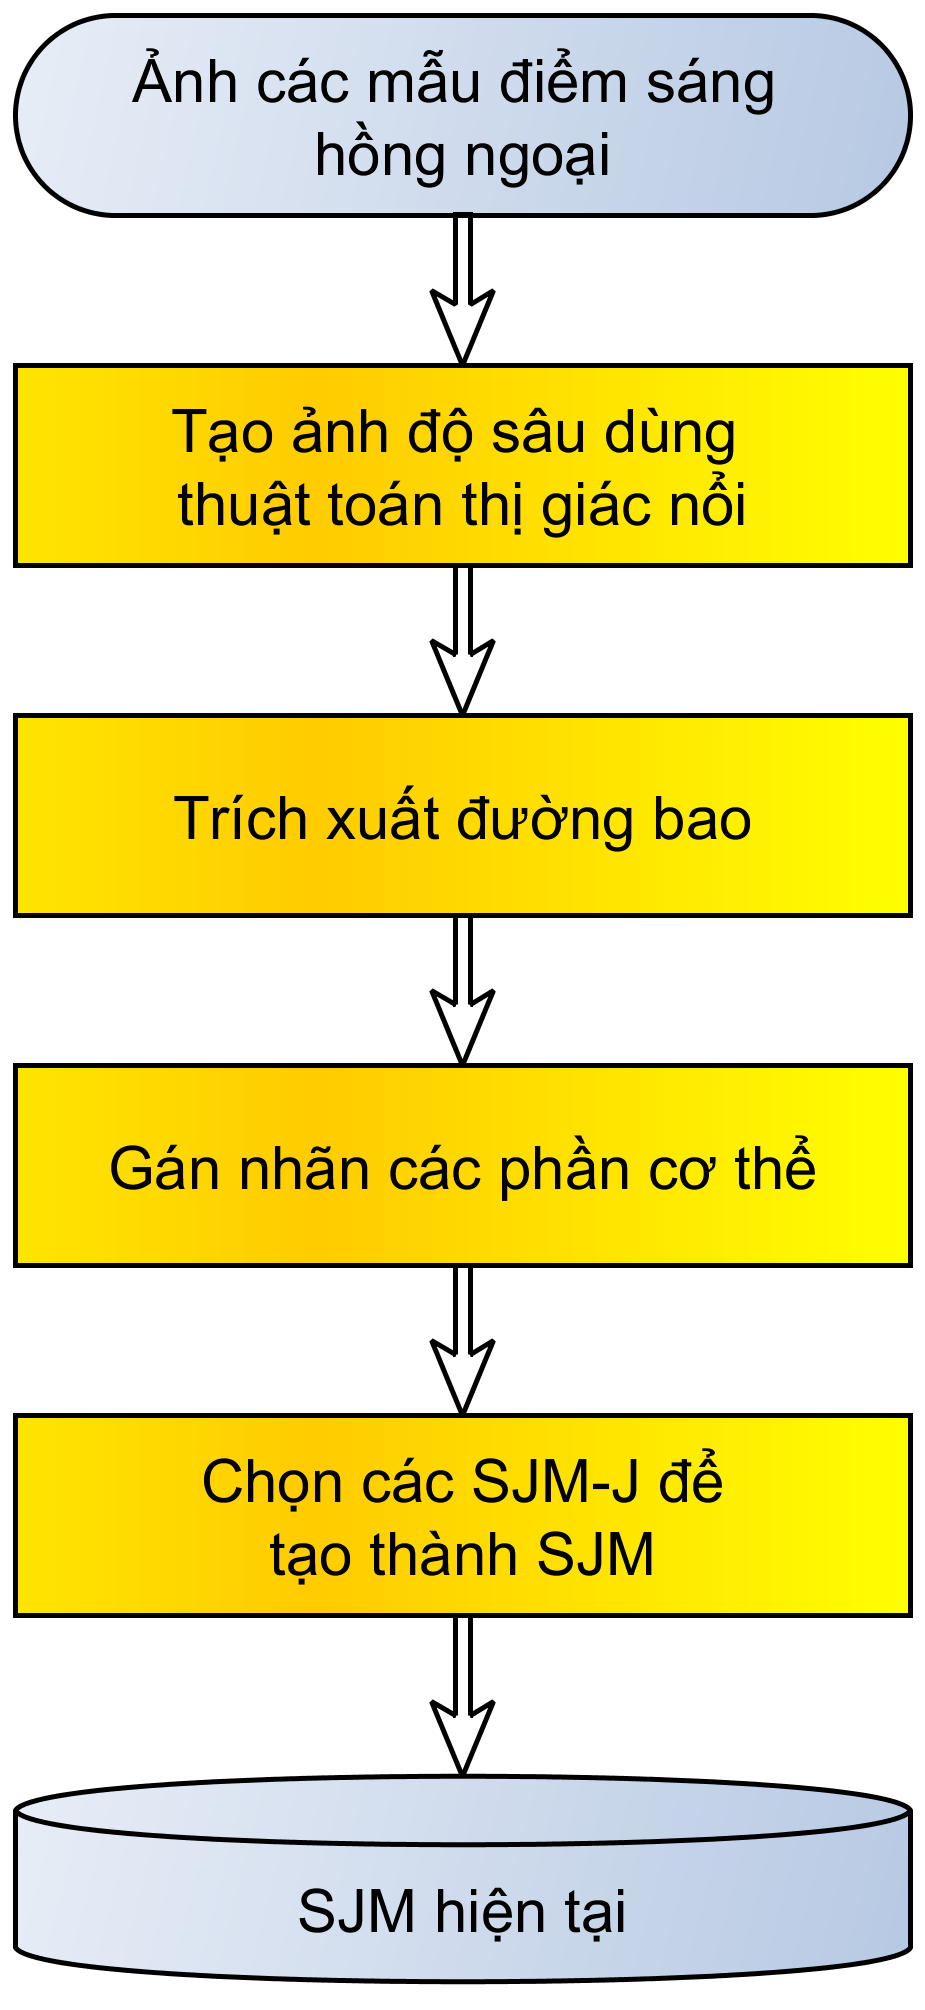
\includegraphics[scale=0.15]{chap3/c3_figs/TrichKhungXuong.png}
\end{center}
\caption{Sơ đồ khối thuật toán trích xuất SJM của thiết bị Kinect \\(Nguồn : "Nhận dạng ngôn ngữ ký hiệu cho người câm" - B.V Phúc, H.C Thịnh)}
\label{fig:TrichKhungXuong}
\end{figure}
\FloatBarrier

\underline{\textbf{Dữ liệu ngõ vào}}

Hành động di chuyển của người dùng trong không gian nhận diện được của thiết bị Kienct v2.

\underline{\textbf{Dữ liệu ngõ ra}}
\begin{itemize}
\item Ảnh màu kých thước 1920x1080 pxs.

\item Ảnh biểu diễn độ sâu 512x424 pxs.

\item SJM tương ứng với ảnh hiện tại biễu diễn tọa độ bằng meter (đo tương đối bằng ảnh độ sâu) hoặc px (tương ứng với vị trí của ảnh độ sâu).
\end{itemize}

Sau khi ước tính tọa độ khung xương bằng Kinect, ta thu được tọa độ các vị trí của 25 khớp xương trong không gian 3 chiều (hình \ref{fig:skeleton_kinect})

\FloatBarrier
\begin{figure}[htp]
\begin{center}
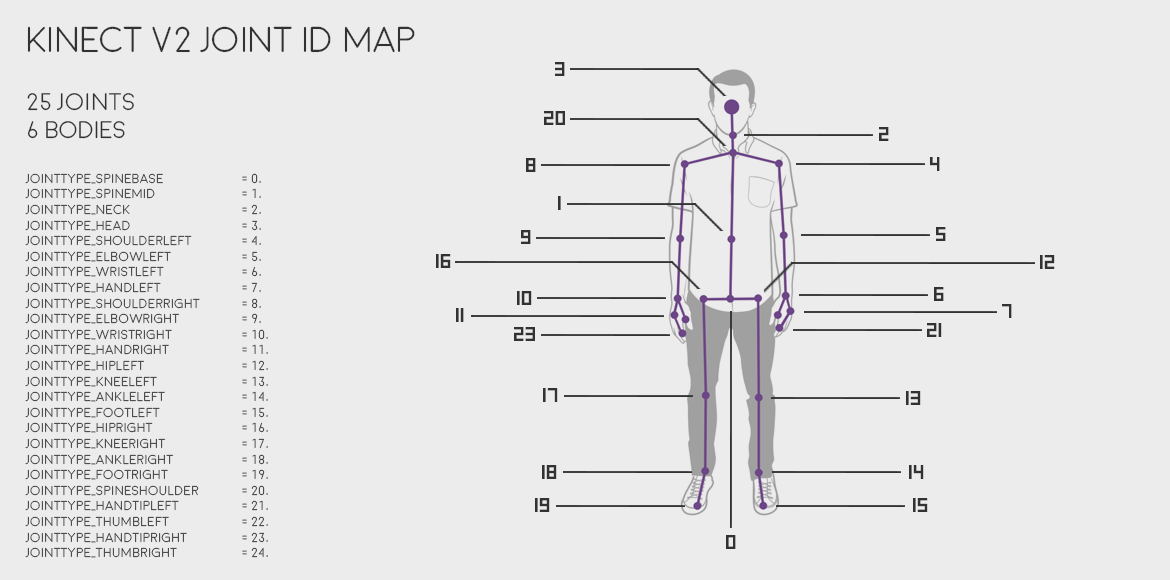
\includegraphics[scale=0.4]{chap3/c3_figs/kinectskeleton.png}
\end{center}
\caption{Khung xương được trích xuất từ Kinect \\(Nguồn : \url{https://www.zonetrigger.com/)}}
\label{fig:skeleton_kinect}
\end{figure}
\FloatBarrier

Việc ước tính tọa độ khung xương dựa trên camera Kinect mang nhiều ưu điểm như tốc độ ước tính nhanh do phần cứng đã tối ưu việc xử lý khớp xương. Kết quả ước tính trên không gian 3 chiều mang độ chính xác cao giúp cho các ứng dụng dựa trên ước tính tọa độ khung xương thực hiện tốt. Tuy nhiên luận văn áp dụng mô hình ước tính tọa độ khung xương dựa vào mạng NN giúp áp dụng vào các thiết bị camera RGB bình thường dễ dàng hơn. Phần tiếp theo luận văn xin trình bày về mạng Neural network này.

\section{ƯỚC TÍNH TỪ ẢNH 2D DỰA TRÊN MẠNG NEURAL NETWORK}
\label{ss:2Dpose}
\subsection{Tổng quan phương pháp}
\label{sss:tong_quan_2D_pose}
Phương pháp trích xuất hình dáng khung xương được áp dụng từ bài báo "Realtime Multi-Person 2D Pose Estimation using Part Affinity Fields" \cite{cao2017realtime} sử dụng phương pháp bottom-up ước tính tọa độ khung xương từ ảnh sang không gian 2D. Tuy có rất nhiều mạng pose estimate cả 2D lẫn 3D và cả dense pose(ước tính toàn bộ hình dáng cơ thể người) nhưng phương pháp ước tính 2D được chọn vì tốc độ xử lý có thể đáp ứng realtime và hoạt động trên các thiết bị cấu hình thấp. Ngoài ra phương pháp này có thể ước tính tọa độ khung xương nhiều người cùng một lúc 

Mạng sử dụng  detect tư thế 2D song song của nhiều người trong một ảnh. Phương pháp sử dụng một đại diện không có thông số "trường ái lực một phần" (PAFs) được tham khảo để học cách liên kết các bộ phần cơ thể với mỗi cá nhân trong ảnh. Mô hình mã hóa toàn bộ bối cảnh, cho phép một bước phân tích từ dưới lên trên (bước này có độ chính xác cao, realtime và thực hiện song song nhiều người). Mô hình được thiết kế để kết hợp tìm vị trí các phần và liên kết giữa chúng thông qua 2 nhánh của quá trình dự đoán chuỗi giống nhau. Phương pháp này đã đạt giải nhất tại cuộc thi COCO 2016 keypoints challenge và vượt trội hơn so với kết quả trước đó trong MPII Multi-Person benchmark về performance và sự hiệu quả.

%\subsection{Kiến trúc mạng}
%\label{sss:method}

\FloatBarrier
\begin{figure}[htp]
\begin{center}
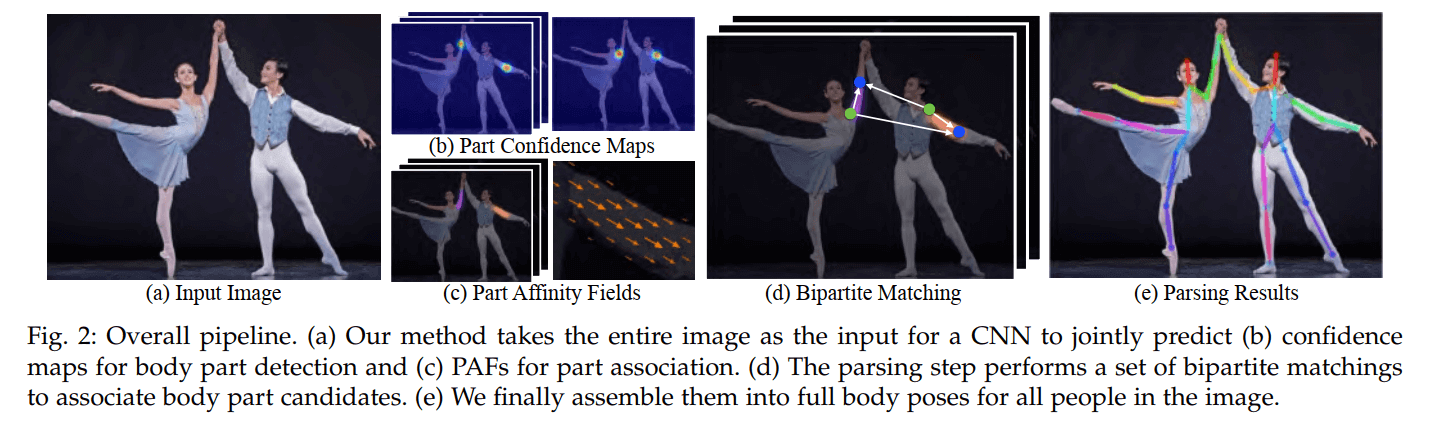
\includegraphics[scale=0.3]{chap3/c3_figs/pipeline.png}
\end{center}
\caption{Tổng thể kiến trúc}
\label{fig:pipeline}
\end{figure}
\FloatBarrier

Hình \ref{fig:pipeline} mình họa toàn bộ nội dung phương pháp. Hệ thống lấy đầu vào, một ảnh màu có kích thước $w*h$ (hình \ref{fig:pipeline}a) và tạo ra ngõ ra, tọa độ của những keyponts cho mỗi cá nhân trong ảnh (hình \ref{fig:pipeline}e). Đầu tiên, một mạng CNN đồng thời dự đoán một loạt những confidence maps (cfm) S của những vị trí bộ phận cơ thể (hình \ref{fig:pipeline}b) và một loạt những miền vector 2D (vf) L của part affinities, cái mà mã hóa độ liên kết giữa các phần cơ thể (hình \ref{fig:pipeline}c). Tập hợp  có J cfm, một map cho mỗi bộ phận, trong đó . Tập hợp  có C vf, một cho mỗi chi, trong đó , mỗi vị trí ảnh trong Lc mã hóa một vector 2D (được show trong hình 1). Cuối cùng, cfm và affinity fields được phân tích bởi suy luận tham lam (hình \ref{fig:pipeline}d) để tạo ra các keypoints 2D cho tất cả người trong ảnh.

Phương pháp này đưa toàn bộ ảnh đầu vào qua một mạng CNN 2 nhánh để đồng thời dự đoán những confidence map cho sự detect phần cơ thể, thể hiện trong hình \ref{fig:pipeline}b, và part affinity fields cho sự liên kết các phần, thể hiện trong hình \ref{fig:pipeline}c. Bước phân tích thể hiện một loạt những liên kết giữa hai điểm (liên kết lưỡng cực) để liên kết những phần cơ thể (\ref{fig:pipeline}d). Cuối cùng, chúng được lắp ráp chúng lại với nhau tạo thành những tư thế cơ thể hoàn chỉnh cho tất cả những người trong ảnh (\ref{fig:pipeline}e).

\begin{itemize} % chấm đầu dòng
\item Đầu tiên, hình ảnh được truyền qua mạng cơ sở để trích xuất các bản đồ đặc trưng. Trong bài báo, tác giả sử dụng 10 lớp đầu tiên của mô hình VGG-19. Tuy nhiên model được luận văn áp dụng sử dụng 10 lớp đầu tiên của mô hình mobilenet\_v2 model này gọn nhẹ hơn so với VGG-19 nên có thể đáp ứng realtime đối với các máy tính cấu hình thấp.
\end{itemize}


\begin{itemize} % chấm đầu dòng
\item Sau đó, các bản đồ tính năng được xử lý với nhiều giai đoạn CNN để tạo: một bộ Bản đồ tin cậy một phần và một bộ các trường có mối quan hệ một phần (PAF)
	\begin{itemize}
	\item \textbf{Confidence Maps} : một bộ bản đồ độ tin cậy 2D S cho các vị trí phần cơ thể. Mỗi vị trí chung có một bản đồ.
	\item \textbf{Part Affinity Fields} : một tập hợp các trường vectơ 2D L mã hóa mức độ liên kết giữa các phần.
	\end{itemize}
\end{itemize}


\begin{itemize} % chấm đầu dòng
\item Cuối cùng, \textbf{Confidence Maps} và \textbf{Part Affinity Fields} được xử lý bằng thuật toán tham lam để có được tư thế cho mỗi người trong ảnh.
\end{itemize}

\subsection{Giải thích các phần}
%\renewcommand{\labelitemi}{$\square$}
%\renewcommand\labelitemii{$\nabla$}
%\renewcommand\labelitemiii{$\square$}
\begin{itemize}
  \item[$\square$] \textbf{Confidence Maps (CFMs)} là một đại diện 2D cho niềm tin rằng một bộ phận cơ thể cụ thể có thể được đặt trong bất kỳ pixel nào. Với J là số lượng vị trí bộ phận cơ thể (khớp). Sau đó, \textbf{Confidence Maps} $S = (S_1, S_2, .., S_J)$ với $S_j \in R^{w \times h},j \in (1 \ldots J)$
  Tóm lại, mỗi bản đồ tương ứng với một khớp và có cùng kích thước với hình ảnh đầu vào .

  \item[$\square$] \textbf{Part Affinity Fields(PAF)}
  Trường quan hệ một phần \textbf{(PAF)} là một tập hợp các trường dòng mã hóa các mối quan hệ cặp đôi không cấu trúc giữa các bộ phận cơ thể.

Mỗi cặp bộ phận cơ thể có một \textbf{PAF} , tức là cổ, mũi, khuỷu tay, v.v.

Cho $C$ là số lượng các cặp phần trên cơ thể. Sau đó \textbf{PAFs} là các thiết lập \textbf{$L = (L_1, L_2, ..., L_c)$} với \textbf{$L_c \in R^{w \times h \times 2},c \in (1 \ldots C)$}

Nếu một pixel nằm trên một chi (phần cơ thể), giá trị trong $L_c$ tại pixel đó là một vectơ đơn vị 2D từ khớp bắt đầu đến khớp cuối.
\item[$\square$] \textbf{CNN nhiều giai đoạn}

\FloatBarrier
\begin{figure}[htp]
\begin{center}
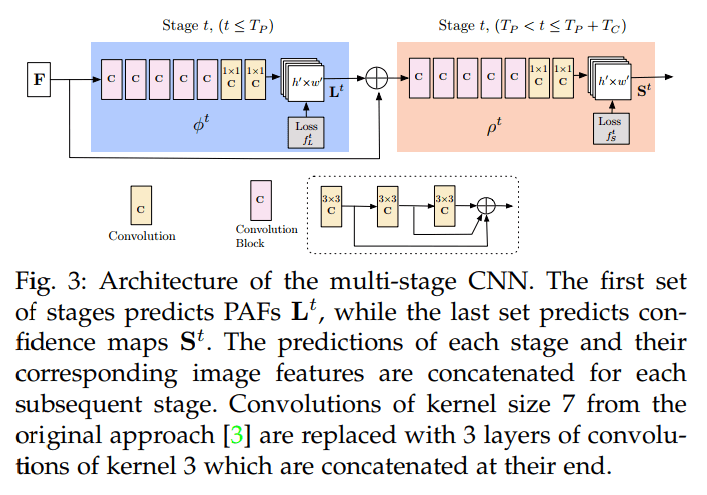
\includegraphics[scale=0.65]{chap3/c3_figs/CNN_m.png}
\end{center}
\caption{Kiến trúc của CNN nhiều giai đoạn từ phiên bản tạp chí của OpenPose}
\label{fig:CNN_multi_stage}
\end{figure}
\FloatBarrier

\textbf{CNN nhiều giai đoạn gồm các bước như sau:}
\begin{itemize}
\item Tính toán các \textbf{part affinity fields (PAFs)}, $ L^{1}$ từ feature maps của mạng cơ sở $F$. Cho $\phi^1$ là mạng CNN mạng CNN tại bước 1. 
$$L^1 = \phi^1(F) $$

\item Giai đoạn $t$ đến giai đoạn $T_P$: Tinh chỉnh dự đoán của \textbf{PAF} từ giai đoạn trước bằng cách sử dụng bản đồ tính năng $F$ và các \textbf{PAF} trước đó $(L^{t-1})$.Với $\phi^t$ là CNN ở giai đoạn t.
$$L^t = \phi^t(F, L^{t-1}), \forall 2 \leq t \leq T_P$$
\item Sau khi $T_P$ lặp đi lặp lại, quá trình được lặp lại việc phát hiện \textbf{confidence maps} , bắt đầu trong dự đoán PAF cập nhật mới nhất . $\rho^t$ là CNN ở giai đoạn $t$. Quá trình được lặp lại cho $T_C$.
$$S^{T_P} = \rho^t(F, L^{T_P}), \forall t = T_P$$
$$S^t = \rho^t(F, L^{T_P}, S^{t-1}), \forall T_P \leq t \leq T_P + T_C$$

\item Ma trận $S$ và $L$ cuối cùng là \textbf{Confidence Maps} và \textbf{part affinity fields (PAFs)} sẽ được xử lý thêm bằng thuật toán tham lam.

\end{itemize}
\end{itemize}
\textbf{Chú thích:}
CNN nhiều giai đoạn này là từ phiên bản tạp chí 2018. Trong phiên bản CVPR 2017 gốc, họ đã tinh chỉnh cả bản đồ độ tin cậy và các trường mối quan hệ một phần (PAF) ở mỗi giai đoạn. Do đó, họ đòi hỏi nhiều tính toán và thời gian hơn ở mỗi giai đoạn. Trong cách tiếp cận mới, tác giả nhận thấy rằng cách tiếp cận mới làm tăng cả tốc độ và độ chính xác tương ứng 200\% và 7\%.

\subsection{Kiến trúc mạng}
\label{sss:structure}
\subsubsection{Phát hiện và liên kết đồng thời}

Kiến trúc của mạng, được show trong hình \ref{fig:structure}, dự đoán đồng thời những cfm và affinity fields \textbf{(af)} cái mà mã hóa liên kết giữa các phần. Mạng được tách thành 2 nhánh: Nhánh trên, màu hường da, dự đoán những \textbf{cfm}, và nhánh dưới, màu xanh, dự đoán những \textbf{af}. Mỗi nhánh là một kiến trúc dự đoán lặp lại, theo như \ref{wei2016convolutional}, nó tinh chỉnh những dự đoán qua các giai đoạn liên tiếp $t \in {{1 \ldots T}}$,  với giám sát trung gian ở từng giai đoạn.

\FloatBarrier
\begin{figure}[htp]
\begin{center}
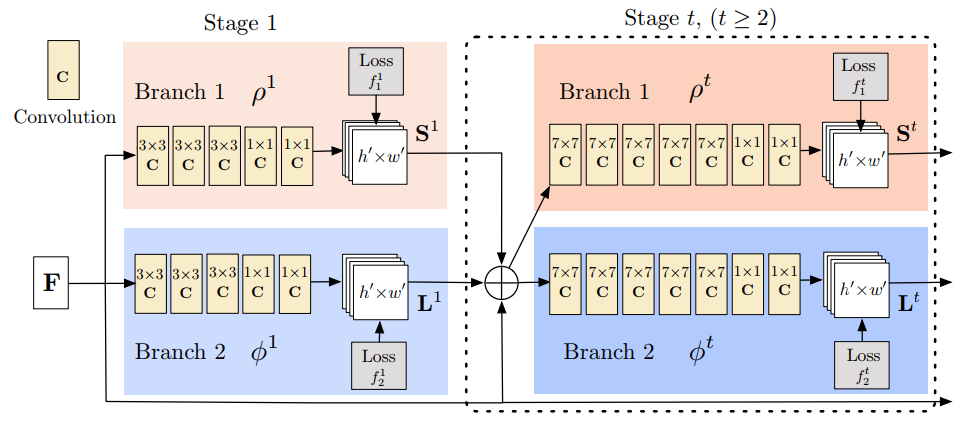
\includegraphics[scale=0.45]{chap3/c3_figs/structure.png}
\end{center}
\caption{Kiến trúc của mạng CNN nhiều bước 2 nhánh. Mỗi bước trong nhánh đầu tiên dự đoán những $CFM S^{t}$, và mỗi bước trong nhánh thứ 2 dự đoán $PAFs L^{t}$. Sau mỗi bước, những dự đoán từ 2 nhánh, cùng với những đặc trưng ảnh, được nối lại cho bước tiếp theo.}
\label{fig:structure}
\end{figure}
\FloatBarrier

\subsection{Phân tích nhiều người sử dụng PAFs}
\label{ss:Multi-Person Parsing using PAFs}

Trong phần này, sẽ nói về tổng quan về thuật toán tham lam được sử dụng để phân tích tư thế của nhiều người từ PAFs và CFMs.

Quá trình phân tích được tóm tắt thành 3 bước sau:
\begin{itemize}
\item Bước 1: Tìm tất cả những vị trí khớp sử dụng confidence maps.
\item Bước 2: Tìm những khớp cùng nhau tạo các chi (bộ phận cơ thể) sử dụng PAFs và những khớp trong bước 1.
\item Bước 3: Kết nối các chi thuộc cùng một người và tạo danh sách những tư thế cơ thể.
\end{itemize}

\subsubsection{Bước 1 - Tìm tất cả những vị trí khớp sử dụng confidence maps.}
\begin{itemize}
\item \textbf{Đầu vào:}
	\begin{itemize}
	\item Confidence maps, $S = (S_1, S_2, .., S_J)$ trong đó $S_j \in R^{w \times h},j \in (1 \ldots J)$.
	\item Up-sampling scale: Sự khác biệt giữa dài/rộng giữa ảnh đầu vào và confidence maps.
	\end{itemize}
\item \textbf{Đầu ra: }
	\begin{itemize}
	\item Danh sách khớp(joints$\_$list): một danh sách những vị trí khớp của kích thước J, mỗi phần tử là một danh sách các đỉnh (x, y, xác suất).
	\item Ví dụ, kích thước của joints$\_$list là 18 cho 18 vị trí khớp (mũi, cổ,...) và những phần tử trong joints$\_$list là những danh sách có độ dài khác nhau. Những phần tử này lưu trữ thông tin đỉnh (vị trí x, y và điểm xác suất) cho mỗi vị trí khớp.
	\end{itemize}
\item \textbf{Xử lý: Cho mỗi khớp từ 1 dến J:}
	\begin{itemize}
	\item Lấy heatmap 2D tương ứng cho khớp trong confidence maps.
	\item Tìm những đỉnh bằng cách lấy ngưỡng heatmap 2D.
	\item Đối với mỗi đỉnh:
		\begin{itemize}
		\item Lấy một đốm xung quanh đỉnh trong heap.
		\item Phóng to đốm sử dụng up-sampling scale.
		\item Lấy vị trí đỉnh lớn nhất trong đốm được phóng to.
		\item Thêm thông tin đỉnh vào danh sách các đỉnh của khớp.
		\end{itemize}
	\end{itemize}
\end{itemize}

\subsubsection{Bước 2 - Tìm những khớp cùng nhau tạo các chi (bộ phận cơ thể) sử dụng PAFs và những khớp trong bước 1.}
\begin{itemize}
\item \textbf{Đầu vào:}
	\begin{itemize}
	\item joints-list ngõ ra của bước 1.
	\item \textbf{PAFs}: \textbf{$L = (L_1, L_2, ..., L_c)$} trong đó \textbf{$L_c \in R^{w \times h \times 2},c \in (1 \ldots C)$}
	\item  Up-sampling scale: sự khác nhau giữa dài rộng của ảnh đầu vào và PAFs maps.
	\item Số lượng những điểm trung gian: số lượng những điểm trung gian giữa một khớp nguồn và những khớp đích để có được giá trị PAFs.
	\end{itemize}
%\end{itemize}
\item \textbf{Đầu ra: }
	\begin{itemize}
	\item Những chi được kết nối (connected-limbs): một danh sách những chi được kết nối có kích thước C. Trong đó, mỗi phần tử là một danh sách tất cả các chi của loại đó.
	\item Mỗi thông tin chi chứa: id của chi nguồn, id của chi đích và điểm số thể hiện độ tốt của kết nối.
	\end{itemize}
\item \textbf{Xử lý: }
	\begin{itemize}
	\item  Phóng to PAFs đến kích thước của ngõ vào sử dụng up-sampling scale.
	\item Đối với mỗi loại chi, ví dụ cổ tay-khuỷu tay trái:
		\begin{itemize}
		\item Lấy tất cả những đỉnh khớp nguồn và những đỉnh khớp đích, ví dụ: tất cả những đỉnh cổ tay trái và tất cả những đỉnh khuỷu tay trái.
		\item Nếu kích thước của những đỉnh nguồn hoặc đỉnh đích bằng 0, thì bỏ qua chi đó.
		\item Tạo một danh sách để lưu trữ tất cả những candidates kết nối chi.
		\item Đối với mỗi đỉnh nguồn và mỗi đỉnh đích:
			\begin{itemize}
			\item Lấy vector trực tiếp bằng cách trừ những vị trí nguồn và vị trí đích.
			\item Chuẩn hóa vector trực tiếp thành vector đơn vị.
			\item  Lấy giá trị PAFs tại mỗi điểm trung gian giữa những đỉnh nguồn và đỉnh đích.
			\item Tính điểm số của kết nối chi hiện tại bằng cách lấy trung bình những giá trị PAFs.
			\item Thêm điểm số để xác định khoảng cách chi phù hợp:  
			
			\textbf{min(0.5 * paf\_height / limb\_dist - 1, 0)}.
			\item Thêm những kết nối chi hiện tại vào những candidates kết nối chi:
			
			+ Sắp xếp những candidates kết nối chi.
			
			+ Đối với mỗi candidate kết nối chi: Thêm sự kết nối vào danh sách cuối cùng nếu nguồn và đích không được chọn cho bất kỳ sự kết nối nào.
			\end{itemize}
		\end{itemize}
	\end{itemize}
\end{itemize}

\subsubsection{Bước 3 - Kết nối các chi thuộc cùng một người và tạo danh sách những tư thế cơ thể.}
\begin{itemize}
\item \textbf{Đầu vào:}
	\begin{itemize}
	\item Danh sách khớp (\textbf{joint$\_$list}) từ bước 1.
	\item Những chi được kết nối (connected$\_$limbs) từ bước 2
	\end{itemize}
\item \textbf{Đầu ra:} Những tư thế: một danh sách những tư thế người cho mỗi các nhân trong ảnh. Mỗi phần từ chứa những vị trí khớp cho người đó.
\item \textbf{Xử lý:}
	\begin{itemize}
	\item Đối với mỗi loại chi và đối với mỗi kết nối giữa các chi (connected\_limbs) của loại đó:
		\begin{itemize}
		\item Tìm những cá nhân liên kết với khớp của kết nối hiện tại.
		\item Nếu không có người nào: Tạo một người mới với kết nối hiện tại.
		\item Nếu có một người: Thêm kết nối hiện tại vào người đó.
		\item Nếu có 2 người: Xác nhập 2 người này thành một người.
		\end{itemize}
	\item Loại bỏ những người có quá ít khớp.
	\end{itemize}
\end{itemize}

\subsection{Kết quả}
Ảnh RGB đầu vào chứa nhiều người sau khi xử lý qua mạng ta nhận được tọa độ 18 khớp xương của từng người được vẽ ra trên ảnh đầu ra. Kết quả ước lượng có thể đáp ứng được xử lý thời gian thực (realtime) trên máy tính cấu hình thấp với FPS đạt được khoảng 2.5 -> 4(FPS). Tốc độ nhận dạng tùy thuộc vào số người trong khung hình, tốc độ xử lý sẽ càng nhanh khi số lượng người trong khung hình càng ít và ngược lại.

\FloatBarrier
\begin{figure}[htp]
\begin{center}
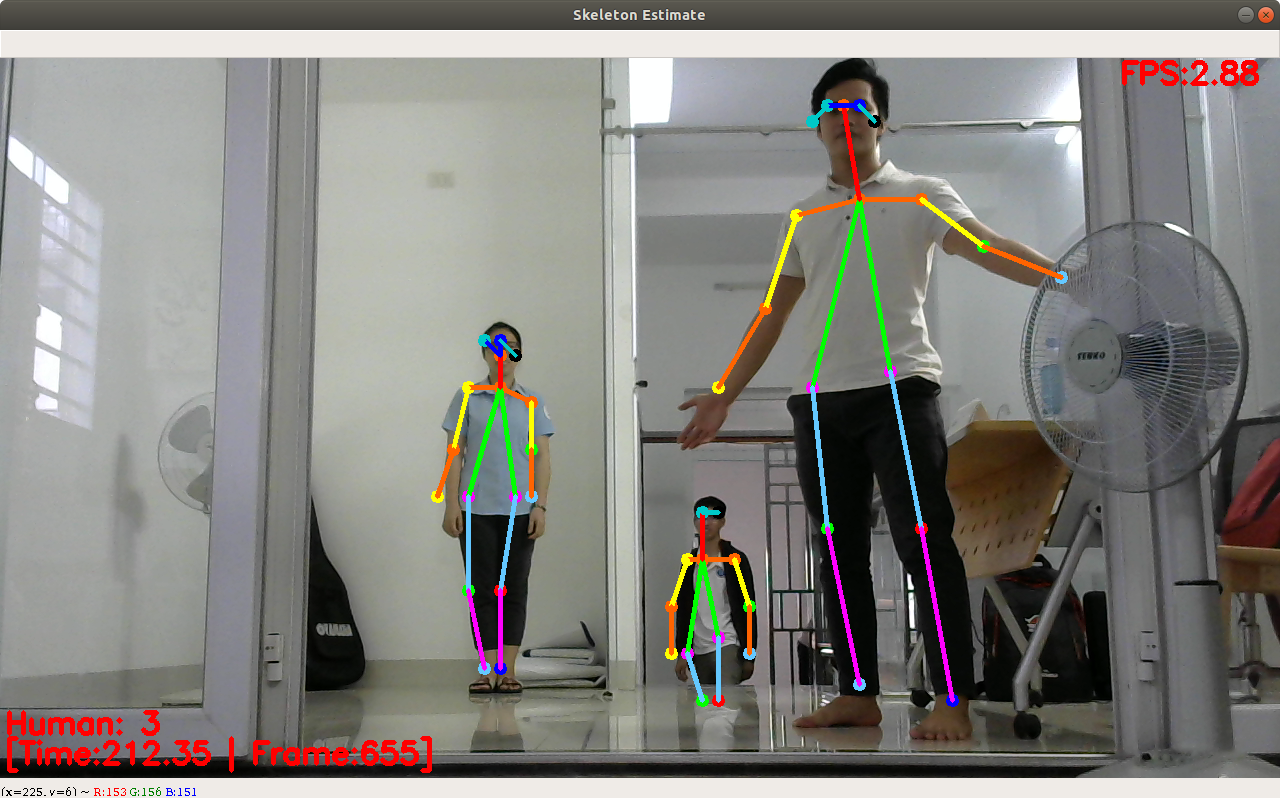
\includegraphics[scale=0.37]{chap3/c3_figs/skeleton_out.png}
\end{center}
\caption{Kết quả ước tính tọa độ khung xương từ mạng NN}
\label{fig:kq_skeleton}
\end{figure}
\FloatBarrier

\section{Kết luận}
Ước lượng khung xương hay ước tính tư thế con người là một hướng nghiên cứu quan trọng và đầy thách thức của thị giác máy tính. Phương pháp này được khá nhiều nghiên cứu áp dụng để giải quyết nhiều bài toán khó như nhận dạng dáng đi, tư thế con người, nhận dạng hành động hay giúp robot học theo chuyển động của con người...Chương tiếp theo, luận văn sẽ trình bày về ứng dụng của ước lượng tọa độ khung xương trong nhận dạng ngôn ngữ ký hiệu, là phần nghiên cứu chính của luận văn.

\newpage
\chapter{XÂY DỰNG MẠNG NEURON NHẬN DẠNG NGÔN NGỮ KÝ HIỆU}
\label{s:DNN}
Trong chương 3, thuật toán ước tính tư thế khung xương đã được trình bày chi tiết về lý thuyết và phương pháp xử lý áp dụng thuật toán. Ta thấy rằng phương pháp này hỗ trợ rất tốt cho việc ước tính nh anhtư thế khung xương trong xử lý thời gian thực. Trong chương 4 này, luận văn sẽ trình bày về đề xuất mô hình mạng DNN lấy đầu vào là toạ độ khung xương được ước tính và nhận dạng cử chỉ thời gian thực. Nội dụng chương trình bày cấu trúc mạng neural network đề xuất, cách thu thập và xử lý dữ liệu cũng như sơ đồ hoạt động chương trinh.
\section{Tổng quan}
Một hành động của con người được đánh giá, xem xét bằng một loạt các cử chỉ theo thời gian. Tuy nhiên, khi xem xét các hành động của con người nhằm tìm ra một cấu trúc nhất quán và có thể tạo thành mô hình thì gặp các vấn đề phức tạp sau:

$\bullet$ Nếu chỉ xem xét đường bao của con người, các phần cơ thể của con người quá gần nhau để có thể xác định được chính xác phần cơ thể cần thiết.

$\bullet$ Hình dạng của cử chỉ (đường bao con người, màu sắc các phần cơ thể), vị trí, loại và kiểu của cử chỉ rất phức tạp. Việc xem xét một mô hình có thể biểu diễn toàn bộ các hành động ngôn ngữ ký hiệu hầu như không thể xem xét nên trong phạm vi luận văn này chỉ xem xét đến việc một mô hình có thể biểu diễn 16 cử chỉ cần sự phối hợp cả hai tay và các cử chỉ tương đối khác nhau (\textbf{Xin chào, Tôi, thành phố, vui vẻ, ẵm em, Sài Gòn, Vĩnh Long, đi bộ, mùa màng, đói bụng, yêu, ăn, biểu quyết, đứng yên, hẹp, rộng}).

$\bullet$ Các hành động của con người có thể giống nhau, tuy nhiên nếu việc quan sát hoặc camera quan sát nằm ở vị trí khác nhau, hướng, độ cao,... đều ảnh hưởng đến khả năng nhận diện hành động của con người. Luận văn đã nêu được phương pháp để có thể phát triển cho việc xác định hành động của con người khi vị trí của camera thay đổi. Tuy nhiên việc kiểm chứng khả năng hoạt động ở các vị trí camera khác nhau sẽ được xem xét ở tương lai.

$\bullet$ Nếu một phần cơ thể bị che khuất bởi các vật thể thì việc xác định hành động của con người sẽ gặp khó khăn hơn rất nhiều so với trường hợp không bị che khuất, phạm vi luận văn không xem xét đến vấn đề này. Tuy nhiên đây là một điểm cần xem xét đến để có thể hoàn thiện hệ thống nhận diện cử chỉ trong tương lai.
\section{Thu thập dữ liệu}
Dữ liệu đầu vào là tọa độ của 18 khớp xương được detect từ mạng mobilenet. Các khớp xương được xuất ra từ mạng được đánh số thứ tự từ 0 tới 17. Các khớp xương cụ thể được thể hiện trong bảng \ref{table:joints} và trong hình \ref{fig:joints}.


\begin{table}[h]
\caption{Các khớp xương được xuất ra từ mạng}
\label{table:joints}
\centering
\begin{center}
\begin{tabular}{|c|p{9cm}|} 
 \hline
Số thứ tự khớp xương  & Vị trí \\
 \hline
 0 & Mũi\\
 \hline 
 1 & Cổ\\
 \hline 
 2 & Vai phải\\
 \hline
 3 & Khủy tay phải \\
 \hline 
 4 & Cổ tay phải\\
 \hline
 5 & Vai trái\\
 \hline
 6 & Khủy trái\\
 \hline
 7 & Cổ tay trái\\
 \hline
 8 & Hông phải\\
 \hline
 9 & Đầu gối phải\\
 \hline
 10 & Cổ chân phải\\
 \hline
 11 & Hông trái\\
 \hline
 12 & Đầu gối trái\\
 \hline
 13 & Cổ chân trái\\
 \hline
 14 & Mắt phải\\
 \hline
 15 & Mắt trái\\
 \hline
 16 & Tai phải\\
 \hline
 17 & Tai trái\\
 \hline
\end{tabular}
\end{center}
\end{table}

\FloatBarrier
\begin{figure}[htp]
\begin{center}
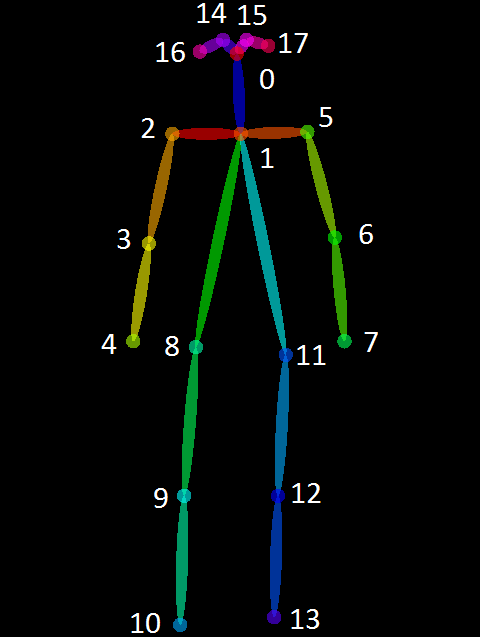
\includegraphics[scale=0.6]{chap4/c4_figs/joints_order.png}
\end{center}
\caption{Sơ đồ khớp xương xuất ra từ mạng mobilenet}
\label{fig:joints}
\end{figure}
\FloatBarrier

Đầu tiên người thu thập dữ liệu đứng trước camera, thực hiện hành động thể hiện từ cần huấn luyện. Chương trình thu thập dữ liệu sẽ xuất ra tọa độ khung xương sau khi xử lý qua mạng pose estimate. Sau đó lưu các tọa độ khớp xương cùng với nhãn của hành động vào file "data.csv" để sau đó đưa vào train. Hình \ref{fig:collect_data} và \ref{fig:collect_data1} thể hiện quá trình khi thu thập dữ liệu.

\FloatBarrier
\begin{figure}[htp]
\begin{center}
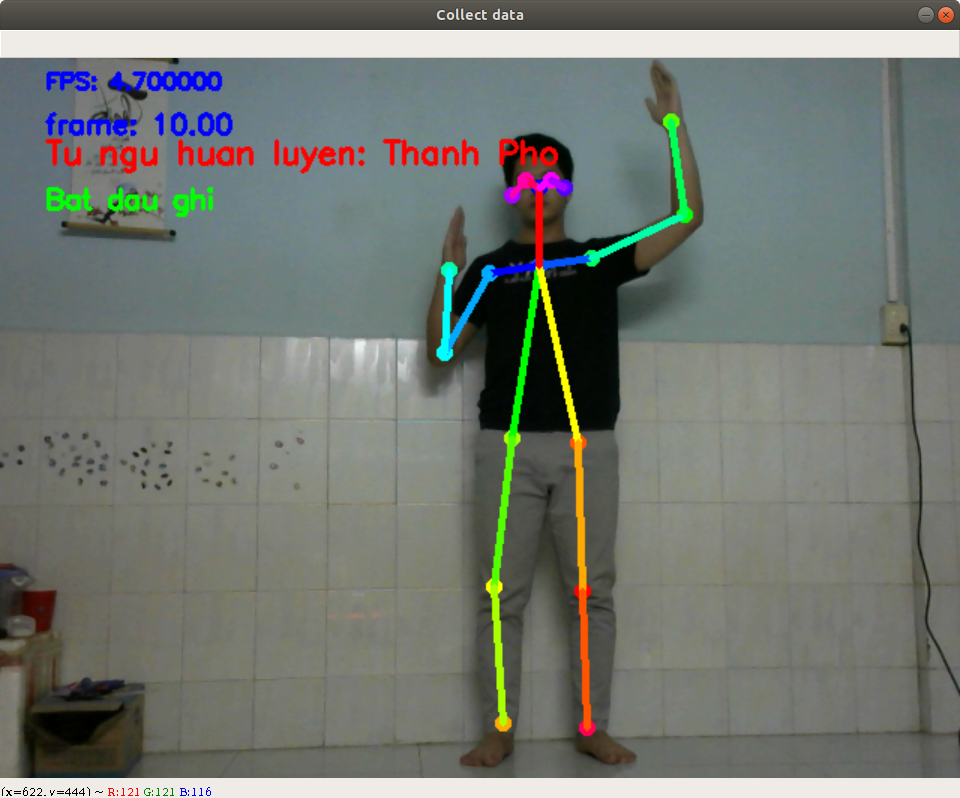
\includegraphics[scale=0.4]{chap4/c4_figs/collect_data.png}
\end{center}
\caption{Giao diện thu thập dữ liệu (khi bắt đầu ghi dữ liệu)}
\label{fig:collect_data}
\end{figure}

\begin{figure}[htp]
\begin{center}
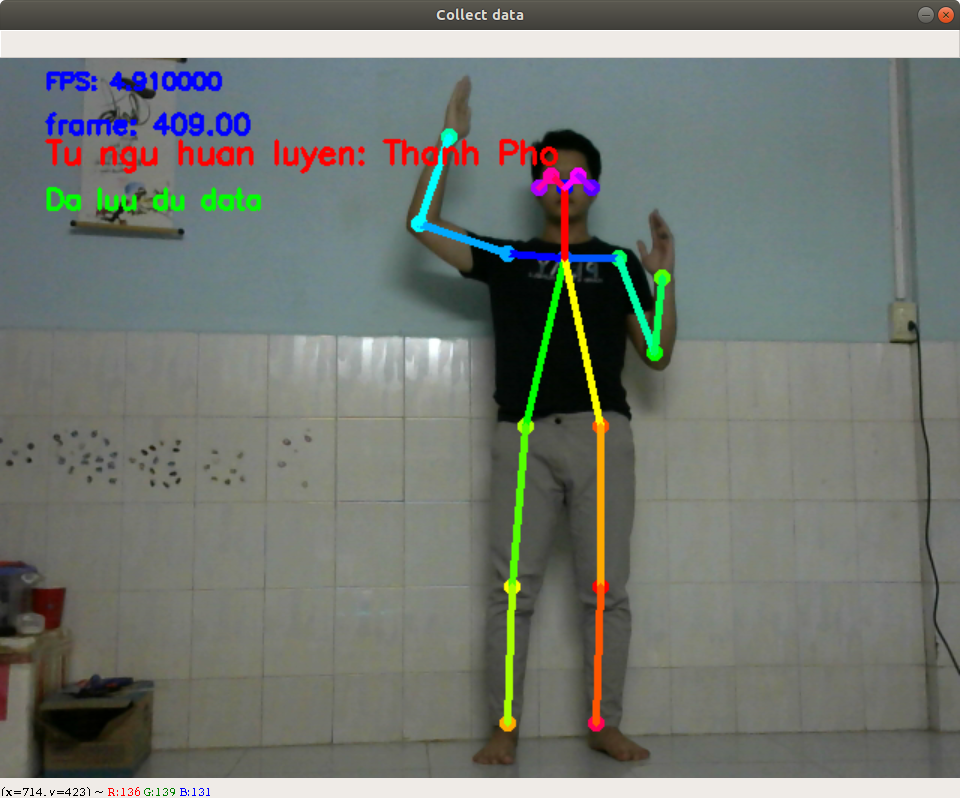
\includegraphics[scale=0.4]{chap4/c4_figs/collect_data1.png}
\end{center}
\caption{Giao diện thu thập dữ liệu (khi đã thu thập đủ dữ liệu)}
\label{fig:collect_data1}
\end{figure}
\FloatBarrier

\section{Xử lý dữ liệu đầu vào}
Dữ liệu sau khi thu thập ban đầu bao gồm tất cả tọa độ các khớp xương ứng các hành động cần nhận dạng. Tuy nhiên khi huấn luyện bộ nhận diện ngôn ngữ ký hiệu ta cần phải xử lý lại dữ liệu khớp xương đã thu thập được. Quá trình xử lý trải qua 2 phần: Loại bỏ các phần khớp xương dư thừa, sau đó chuẩn hóa lại các vector SJM.

\subsection{Loại bỏ các phần SJM dư thừa}
Ngôn ngữ ký hiệu với đặc trưng là sự phối hợp phần trên cơ thể với hai tay để diễn đạt từ ngữ mong muốn. Do đó việc xem xét đến các khớp xương phần dưới cơ thể là không cần thiết. Phần xử lý này, đề tài đã loại bỏ các tọa độ SJM dư thừa, chỉ giữ lại 10 điểm khớp xương cần thiết cho việc nhận diện: \textbf{Mũi, Cổ, Vai trái, khuỷu tay trái, Cổ tay trái, Vai phải, Khủy tay phải, Cổ tay phải, hông phải và hông trái} như thể hiện trong hình \ref{fig:joints} và bảng \ref{table:joints_choose}

\FloatBarrier
\begin{figure}[htp]
\begin{center}
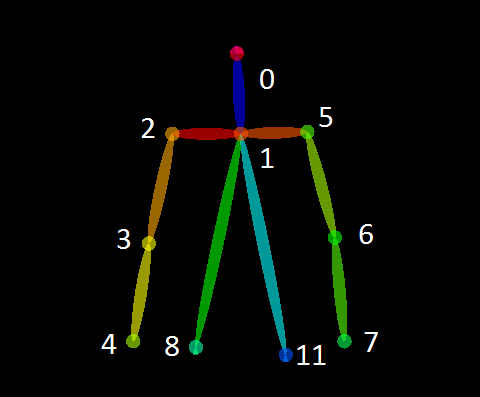
\includegraphics[scale=1]{chap4/c4_figs/joints_choose.png}
\end{center}
\caption{Sơ đồ khớp xương sau khi loại bỏ các phần không cần thiết}
\label{fig:joints}
\end{figure}
\FloatBarrier

\FloatBarrier
\begin{table}[h]
\caption{Các khớp xương được giữ lại}
\label{table:joints_choose}
\centering
\begin{center}
\begin{tabular}{|c|p{9cm}|} 
 \hline
Số thứ tự khớp xương  & Vị trí \\
 \hline
 0 & Mũi\\
 \hline 
 1 & Cổ\\
 \hline 
 2 & Vai phải\\
 \hline
 3 & Khủyu tay phải \\
 \hline 
 4 & Cổ tay phải\\
 \hline
 5 & Vai trái\\
 \hline
 6 & Khủyu tay trái\\
 \hline
 7 & Cổ tay trái\\
 \hline
 8 & Hông phải\\
 \hline
 11 & Hông trái\\
 \hline
\end{tabular}
\end{center}
\end{table}
\FloatBarrier

\subsection{Chuẩn hóa SJM để phân loại đặc trưng}

Dựa vào dữ liệu thu thập được, ta có thể nhận thấy là tùy vào vị trí camera, khoảng cách từ camera đến người được quan sát sẽ làm thay đổi giá trị của các vector khung xương SJM. Hình \ref{fig:kq_skeleton} từ kết quả chương 3 có thể thấy khoảng cách các SJM của người ở xa camera sẽ gần nhau hơn so với người ở gần. Do đó cần phải sử dụng phương pháp chuẩn hóa dữ liệu các vector, đưa các vector đặc trưng SJM về cùng kích cỡ thì dữ liệu đưa vào train mới có thể có cùng những đặc trưng giống nhau.

Phương pháp chuẩn hóa được áp dụng như sau:


Đầu tiên, ta sử dụng các dữ liệu ban đầu - raw data cho việc gán đặc trưng. Xem xét bảng vị trí của các SJM-J trong một SJM đặc trưng từ bảng \ref{BangSJM}.

\begin{table}[htbp]
\centering
\caption{Một SJM đặc trưng nhận được từ quá trình thí nghiệm}
\begin{tabular}{|c|c|c|}
\hline 
 Điểm SJM-J & Tên SJM-J & $(x_i; y_i) $\\ 
\hline 
A & Mũi  & (992.574; 411.311) \\
\hline 
B & Vai trái & (987.327; 519.09) \\ 
\hline 
C & Vai phải  & (987.795; 783.878) \\ 
\hline 
D & Cổ tay trái & (870.784; 666.671) \\ 
\hline 
E & Cổ tay phải & (826.394; 825.466) \\ 
\hline
F & Khuỷu tay trái & (1114.381; 662.63) \\ 
\hline
G & Khuỷu tay phải & (1174.36; 825.96) \\ 
\hline 
\end{tabular} 
\label{BangSJM}
\end{table}

Các vector của SJM có thể được biểu diễn:
\begin{equation}
v_n=(x_n; y_n; z_n)
\end{equation}
Trong đó: $(x_n; y_n; z_n)$: tọa độ các SJM-J đang xét tới.

Với các tính toán vector như trên, từ 7 SJM-J có được 6 vectors biễu diễn SJM. Vấn đề xảy ra khi sử dụng 4 vectors này để tính toán đặc trưng, 6 vectors này có tọa độ trong không gian ba chiều sẽ khiến cho việc mô hình hóa khó khăn hơn. Do đó, ta chuyển đổi 6 vectors này từ không gian ba chiều xuống không gian hai chiều. Xem xét việc trong quá trình hoạt động thể hiện hành động ta luôn đứng hướng thẳng mặt vào camera, do đó khoảng cách tối đa trên trục z (khoảng cách đến anten ) giữa các SJM-J là không lớn nên tất cả các SJM-J được chiếu lên trục z.

Chiếu các vector khung xương lên trục z ta có được các vector mới:
\begin{equation}
v'_n = ({x_n}; {y_n})
\end{equation}

Để có thể tính toán tổng bình phương khoảng cách chuẩn hóa thì ta phải xoay và thay đổi độ dài của các vector sao cho vector khung xương được tạo ra giữa hai SJM-J cột sống trở thành vector đơn vị - unit vector:
\begin{equation}
v_\textit{spin-shouder} = (0;1)
\end{equation}

Ta có tọa độ vị trí các SJM-J sau khi chuẩn hóa:\*

\begin{tabular}{c c c}
A(992.574; 411.311) & $\Rightarrow$ & ... \\ 
B(987.327; 519.09) & $\Rightarrow$ & B(0;1) \\ 
C(987.795; 783.878) & $\Rightarrow$ & C(0;0) \\ 
D(870.784; 666.671) & $\Rightarrow$ & ... \\ 
E(826.394; 825.466) & $\Rightarrow$ & ... \\ 
F(1114.381; 662.63) & $\Rightarrow$ & ... \\ 
G(1174.36; 825.96) & $\Rightarrow$ & ... \\ 
\end{tabular} \*

Công thức để tính toán vị trí mới, chuẩn hóa của A, B, C, D, E, F, G:

\begin{equation}
{y_{A'}} = \frac{1}{2}\left( {{{\left( {\frac{{AC}}{{BC}}} \right)}^2} - {{\left( {\frac{{AB}}{{BC}}} \right)}^2} + 1} \right) = \frac{{A{C^2} - A{B^2} + B{C^2}}}{{2B{C^2}}}
\end{equation}

Một hàm tính toán được thêm vào để dễ dàng lập trình hơn:
\begin{equation}
{f_{BC}}(x,y) = ({y_B} - {y_C})x - ({x_B} - {x_c})y - ({y_B} - {y_C}){x_C} + ({x_B} - {x_c}){y_C}
\end{equation}

với đặc điểm:\\

$\bullet \text{   }  f_\text{BC}(x_A,y_A > 0$: điểm A nằm phía trên đoạn thẳng BC\\

$\bullet \text{   }  f_\text{BC}(x_A,y_A)< 0$: điểm A nằm phía dưới đoạn thẳng BC\\

$\bullet \text{   } f_\text{BC}(x_A,y_A)= 0$: điểm A nằm trên đường thẳng chứa đoạn thẳng BC\\

Hàm BC không có ý nghĩa hình học tuy nhiên lại có ý nghĩa về mặt đại số, dựa vào hàm kết quả vị trí tương đối giữa điểm A và BC, ta có thể tìm được giá trị của $x_\text{A'}$ :

\begin{equation}
{x_{A'}} = {\mathop{\rm sgn}} ({f_{BC}}({x_A},{y_A})\sqrt {{{\left( {\frac{{AC}}{{BC}}} \right)}^2} - {y_{A'}}^2} 
\end{equation}

Tương tự với vị trí $D_0, E_0, F_0, G_0$ với điểm gốc là B,C. Sau khi tìm được $A_0, B_0, C_0, D_0, E_0, F_0, G_0$ ta có được 6 vectors đặc trưng tương ứng với $SJM_i$ như sau:

\begin{tabular}{c c}
$\overrightarrow {{v_{i,1}}}  = \overrightarrow {C'A'}  = $&$({x_{A'}};{y_{A'}})$ \\ 
$\overrightarrow {{v_{i,0}}}  = \overrightarrow {C'B'}  = $&$(0;1)$ \\ 
$\overrightarrow {{v_{i,2}}}  = \overrightarrow {C'D'}  = $&$({x_{D'}};{y_{D'}})$ \\ 
$\overrightarrow {{v_{i,3}}}  = \overrightarrow {C'E'}  = $&$({x_{E'}};{y_{E'}})$ \\ 
$\overrightarrow {{v_{i,4}}}  = \overrightarrow {C'F'}  = $&$({x_{F'}};{y_{F'}})$ \\ 
$\overrightarrow {{v_{i,5}}}  = \overrightarrow {C'G'}  = $&$({x_{G'}};{y_{G'}})$ \\ 


\end{tabular} 

Áp dụng cách tính toán trên vào bảng \ref{BangSJM}, ta được tọa độ 6 vector đặc trưng của các $SJM_i$ tương ứng và minh họa trên hình \ref{figure48}:

\begin{table}[htbp]
\centering
\caption{Một SJM đặc trưng sau khi chuẩn hóa}
\begin{tabular}{|c|c|c|}
\hline 
 Điểm SJM-J & Tên SJM-J & $(x_i; y_i) $\\ 
\hline 
A & Đầu  & (0.0205352100186477; -0.407002543626264) \\ 
\hline 
B & Cột sống vai & (0; 0) \\ 
\hline 	
C & Cột sống gốc & (0; 1) \\ 
\hline 
D & Khuỷu tay trái & (-0.441120735865053; 0.55657565862356) \\ 
\hline 
E & Bàn tay trái & (-0.60982370936332; 1.15598366430513) \\ 
\hline
F & Khuỷu tay phải & (0.478873301943448; 0.542940438030838) \\ 
\hline
G & Bàn tay phải & (0.704299437754533; 1.16017195694997) \\ 
\hline 
\end{tabular} 
\label{BangSJMResult}
\end{table}


    \begin{figure}[htp]
    \begin{center}
     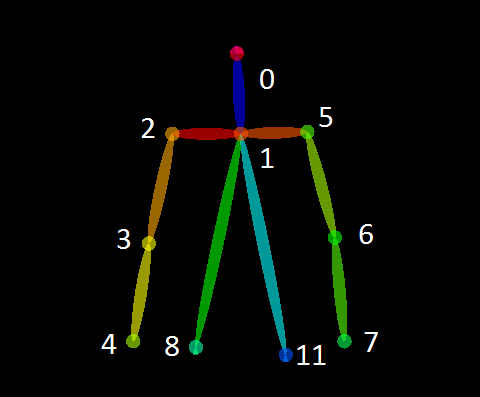
\includegraphics[scale=0.6]{chap4/c4_figs/joints_choose.png}
    \end{center}
    \caption{SJM sau chuẩn hóa} 
    \label{figure48}
    \end{figure}



Giá trị bình phương sai lệch khoảng cách giữa hai $SJM_i$ và $SJM_j$ đã chuẩn hóa mang ý nghĩa là giá trị khác biệt giữa hai SJMs:

\begin{equation}
{\Delta _{ij}} = \sum\limits_{k = 1}^5 {\parallel \overrightarrow {{v_{i,k}}}  - \overrightarrow {{v_{j,k}}} \parallel } 
\label{equ3.8}
\end{equation}




Sau khi loại bỏ các phần thừa và chuẩn hóa hết bộ dữ liệu các SJM, ta được các SJM với tọa độ các điểm khớp xương được chuẩn hóa nằm trong khoảng 0 --> 1 thể hiện trong hình \ref{fig:skeleton_normalize}
\FloatBarrier
\begin{figure}[htp]
\begin{center}
\includegraphics[scale=0.25]{chap4/c4_figs/datajoint.png}
\end{center}
\caption{Dữ liệu khớp xương sau khi đã được chuẩn hóa}
\label{fig:skeleton_normalize}
\end{figure}
\FloatBarrier

\section{Cấu trúc mạng neural network xây dựng}
Từ dữ liệu đầu vào là một ảnh RGB, qua bước phát hiện khung xương với mạng CNN và các bước chuẩn hóa, loại bỏ khớp xương thừa, dữ liệu cần phân loại gần như đã lấy ra hết đặc trưng cần tìm và giảm số chiều đến tối đa. Do đó mạng DNN cần dùng để phân loại các từ ngôn ngữ ký hiệu chỉ cần một cấu trúc vừa phải và giảm thiểu số trọng số đến tối đa.
\begin{itemize}
\item Input: Mạng với đầu vào là 20 nodes ứng với tọa độ của 10 khớp xương (mỗi khớp là 2 tọa độ).
\item Hidden layer: Là các lớp Fully connected (Dense) và Normalization xen kẽ nhau.
\item Output: Với softmax với 16 nodes ứng với 16 từ ngữ nhận diện được.
\end{itemize}
Cụ thể các thông số và cấu trúc được thể hiện trong hình \ref{fig:model_params}.

\FloatBarrier
\begin{figure}[htp]
\begin{center}
\includegraphics[scale=1.3]{chap4/c4_figs/model_param.png}
\end{center}
\caption{Các thông số của mạng DNN}
\label{fig:model_params}
\end{figure}
\FloatBarrier


Model sử dụng khá nhiều lớp Batch Normalization. Về lý thuyết toán thì layer này có tác dụng trong 2 việc đó là:
\begin{itemize}
\item Tránh gradient tiến về 0 sẽ chẳng biết là đi lên hay xuống.
\item Gradient quá lớn khiến các tham số không thể tối ưu được (loss sẽ nhảy lung tùng).
\end{itemize}
Cụ thể là nó giúp chuẩn hóa dữ liệu về 1 khoảng (0,1).

\section{Huấn luyện mạng}
Mạng được huấn luyện theo thuật toán Stochastic Gradient Descent (SGD) là một biến thể của Gradient Descent. Cụ thể ta sẽ tìm hiểu về nó qua các phần dưới dây.

\subsection{Gradient Descent}
Trong Machine Learning nói riêng và Toán Tối Ưu nói chung, chúng ta thường xuyên phải tìm giá trị nhỏ nhất (hoặc đôi khi là lớn nhất) của một hàm số nào đó. Ví dụ như các hàm mất mát trong hai bài Linear Regression và K-means Clustering. Nhìn chung, việc tìm global minimum của các hàm mất mát trong Machine Learning là rất phức tạp, thậm chí là bất khả thi. Thay vào đó, người ta thường cố gắng tìm các điểm local minimum, và ở một mức độ nào đó, coi đó là nghiệm cần tìm của bài toán.

Các điểm local minimum là nghiệm của phương trình đạo hàm bằng 0. Nếu bằng một cách nào đó có thể tìm được toàn bộ (hữu hạn) các điểm cực tiểu, ta chỉ cần thay từng điểm local minimum đó vào hàm số rồi tìm điểm làm cho hàm có giá trị nhỏ nhất. Tuy nhiên, trong hầu hết các trường hợp, việc giải phương trình đạo hàm bằng 0 là bất khả thi. Nguyên nhân có thể đến từ sự phức tạp của dạng của đạo hàm, từ việc các điểm dữ liệu có số chiều lớn, hoặc từ việc có quá nhiều điểm dữ liệu.

Hướng tiếp cận phổ biến nhất là xuất phát từ một điểm mà chúng ta coi là gần với nghiệm của bài toán, sau đó dùng một phép toán lặp để tiến dần đến điểm cần tìm, tức đến khi đạo hàm gần với 0. Gradient Descent (viết gọn là GD) và các biến thể của nó là một trong những phương pháp được dùng nhiều nhất.

Các bước quan trọng của thuật toán Gradient Descent như sau:
\begin{itemize}
\item Dự đoán một điểm khởi tạo $\theta = \theta_0$.
\item Cập nhật $\theta$ đến khi đạt được kết quả chấp nhận được: 
$$\theta = \theta - \eta \nabla_{\theta}J(\theta)$$
với $\nabla_{\theta}J(\theta)$ là đạo hàm của hàm mất mát tại $\theta$
\end{itemize}

\textbf{Gradient dưới góc nhìn vật lý:}

Thuật toán GD thường được ví với tác dụng của trọng lực lên một hòn bi đặt trên một mặt có dạng như hình một thung lũng giống như hình \ref{fig:gradient} dưới đây. Bất kể ta đặt hòn bi ở A hay B thì cuối cùng hòn bi cũng sẽ lăn xuống và kết thúc ở vị trí C.

\FloatBarrier
\begin{figure}[htp]
\begin{center}
\includegraphics[scale=0.06]{chap4/c4_figs/momentum.png}
\end{center}
\caption{So sánh Gradient Descent với các hiện tượng vật lý (Nguồn: "Machine learning cơ bản" - Vũ Hữu Tiệp)}
\label{fig:gradient}
\end{figure}
\FloatBarrier

Tuy nhiên, nếu như bề mặt có hai đáy thung lũng như Hình \ref{fig:gradient}b thì tùy vào việc đặt bi ở A hay B, vị trí cuối cùng của bi sẽ ở C hoặc D. Điểm D là một điểm local minimum chúng ta không mong muốn.

Nếu suy nghĩ một cách vật lý hơn, vẫn trong Hình \ref{fig:gradient}b, nếu vận tốc ban đầu của bi khi ở điểm B đủ lớn, khi bi lăn đến điểm D, theo đà, bi có thể tiếp tục di chuyển lên dốc phía bên trái của D. Và nếu giả sử vận tốc ban đầu lớn hơn nữa, bi có thể vượt dốc tới điểm E rồi lăn xuống C như trong Hình \ref{fig:gradient}c. Đây chính là điều chúng ta mong muốn.

\subsection{Stochastic Gradient Descent}
Trong thuật toán này, tại 1 thời điểm, ta chỉ tính đạo hàm của hàm mất mát dựa trên chỉ một điểm dữ liệu $\mathbf{x_i}$ rồi cập nhật 
$\theta$ dựa trên đạo hàm này. Việc này được thực hiện với từng điểm trên toàn bộ dữ liệu, sau đó lặp lại quá trình trên. Thuật toán rất đơn giản này trên thực tế lại làm việc rất hiệu quả.

Mỗi lần duyệt một lượt qua tất cả các điểm trên toàn bộ dữ liệu được gọi là một epoch. Với GD thông thường thì mỗi epoch ứng với 1 lần cập nhật $\theta$, với SGD thì mỗi epoch ứng với $\mathbf{N}$ lần cập nhật $\mathbf{\theta}$ với $\mathbf{N}$ là số điểm dữ liệu. Nhìn vào một mặt, việc cập nhật từng điểm một như thế này có thể làm giảm đi tốc độ thực hiện 1 epoch. Nhưng nhìn vào một mặt khác, SGD chỉ yêu cầu một lượng epoch rất nhỏ (thường là 10 cho lần đầu tiên, sau đó khi có dữ liệu mới thì chỉ cần chạy dưới một epoch là đã có nghiệm tốt). Vì vậy SGD phù hợp với các bài toán có lượng cơ sở dữ liệu lớn (chủ yếu là Deep Learning mà chúng ta sẽ thấy trong phần sau của blog) và các bài toán yêu cầu mô hình thay đổi liên tục, tức online learning.

\textbf{Thứ tự lựa chọn điểm dữ liệu:}
Một điểm cần lưu ý đó là: sau mỗi epoch, chúng ta cần shuffle (xáo trộn) thứ tự của các dữ liệu để đảm bảo tính ngẫu nhiên. Việc này cũng ảnh hưởng tới hiệu năng của SGD.

Một cách toán học, quy tắc cập nhật của SGD là:
$$\theta = \theta - \eta \nabla_{\theta} J(\theta; \mathbf{x}_i; \mathbf{y}_i)$$
trong đó $J(\theta; \mathbf{x}_i; \mathbf{y}_i)$ là hàm mất mát với chỉ 1 cặp điểm dữ liệu (input, label) là $(\mathbf{x}_i, \mathbf{y}_i)$. Ngoài ra, chúng ta hoàn toàn có thể áp dụng các thuật toán tăng tốc GD như Momentum, AdaGrad,… vào SGD.

\subsection{Điều kiện dừng}
Trong thực nghiệm, có một vài phương pháp như dưới đây để xác định khi nào cần dừng số vòng lặp khi huấn luyện:
\begin{itemize}
\item Giới hạn số vòng lặp: đây là phương pháp phổ biến nhất và cũng để đảm bảo rằng chương trình chạy không quá lâu. Tuy nhiên, một nhược điểm của cách làm này là có thể thuật toán dừng lại trước khi đủ gần với nghiệm.
\item So sánh gradient của nghiệm tại hai lần cập nhật liên tiếp, khi nào giá trị này đủ nhỏ thì dừng lại. Phương pháp này cũng có một nhược điểm lớn là việc tính đạo hàm đôi khi trở nên quá phức tạp (ví dụ như khi có quá nhiều dữ liệu), nếu áp dụng phương pháp này thì coi như ta không được lợi khi sử dụng SGD và mini-batch GD.
\item So sánh giá trị của hàm mất mát của nghiệm tại hai lần cập nhật liên tiếp, khi nào giá trị này đủ nhỏ thì dừng lại. Nhược điểm của phương pháp này là nếu tại một thời điểm, đồ thị hàm số có dạng bẳng phẳng tại một khu vực nhưng khu vực đó không chứa điểm local minimum (khu vực này thường được gọi là saddle points), thuật toán cũng dừng lại trước khi đạt giá trị mong muốn.
\item Trong SGD và mini-batch GD, cách thường dùng là so sánh nghiệm sau một vài lần cập nhật.
\end{itemize}


\subsection{Áp dụng vào bài toán}
Với bộ dữ liệu của bài toán nhận dạng ngôn ngữ ký hiệu, dữ liệu là các SJM được thu thập từ trước. Dữ liệu sẽ được chia ra thành 2 tập gồm: train data (dữ liệu để huấn luyện) và test data (dữ liệu đánh giá) với tỷ lệ 80 và 20. Nghĩa là với mỗi hành động (data gồm 800 SJM) sẽ có 640 SJM để train và 160 SJM để đánh giá.
Áp dụng thuật toán SGD, với các thông số ban đầu được khởi tạo trước khi huấn luyện như sau:
\begin{itemize}
\item epoch: 50
\item learning rate: 0.0001
\item batch$\_$size : 32
\end{itemize}
Trong quá trình huấn luyện, luận văn sử dụng phương pháp lưu lại checkpoint. Cách thức hoạt động của phương pháp này là sau mỗi epoch, accuracy trên tập test của model hiện tại được so sánh với accuracy của model trước đó. Nếu nó lớn hơn thì trọng số của mô hình sẽ được cập nhật theo trọng số mới nhất. Nếu nhỏ hơn, trọng số của mô hình trước đó vẫn được giữ lại cho đến khi accuracy khác cao hơn. Phương pháp này giúp tìm được model tối ưu nhất với accuracy cao nhất có thể.
Sau 50 epoch, ta có kết quả về độ chính xác(accuracy) và sai số (loss) trên tập train và tập test như sau:
\FloatBarrier
\begin{figure}[htp]
\begin{center}
\includegraphics[scale=1]{chap4/c4_figs/train_val_acc.png}
\end{center}
\caption{Accurracy của tập train và validate}
\label{fig:pipelineS}
\end{figure}
\FloatBarrier

\FloatBarrier
\begin{figure}[htp]
\begin{center}
\includegraphics[scale=1]{chap4/c4_figs/train_val_l.png}
\end{center}
\caption{Loss của tập train và validate}
\label{fig:pipelineS}
\end{figure}
\FloatBarrier

Từ biểu đồ accuracy và loss của mô hình, có thể thấy mô hình đã học được rất tốt. Kể từ epoch thứ 10, mô hình đã đạt được accuracy cao và loss giảm xuống thấp. Đường biểu diễn của 2 tập đối với accuracy và loss đi sát nhau có thể phần nào dự đoán được mô hình không bị overfiting. 

\section{Kết quả}

Nhận thấy kết quả mô hình đã học được rất tốt với thuật toán này. Với kết quả cuối cùng:
\begin{itemize}
\item Train Accuracy: 1.0000
\item Test Accuracy: 0.9996
\item Train Loss: 0.0153
\item Test Loss    : 0.0123
\end{itemize}

Dựa vào những thông số trên có thể thấy kết quả sau khi huấn luyện mô hình khá tốt. Nhưng để áp dụng mô hình vào thực tế được, ta cần phải thử nghiệm và đánh giá bằng nhiều phương pháp trên tập dữ liệu mới. Trong chương 5 luận văn sẽ trình bày về cách thức thử nghiệm, đánh giá mô hình cũng như xây dựng phần mềm ứng dụng từ mô hình.  Chương 4 tiếp theo luận văn sẽ trình bày giải thuật Deep Sort dùng để theo dõi những người trong khung ảnh, từ đó có thể áp dụng nhận diện dc chuỗi các ký tự của ngôn ngữ ký hiệu mà từng người diễn đạt.
















\newpage
\chapter{Giải thuật Deep Sort theo dõi từng người trong khung hình}
Qua các chương trước, luận văn đã trình bày thuật toán, lý thuyết cũng nhhư cách thức hoạt động của chương trình nhận dạng ngôn ngữ ký hiệu. Ở chương này, luận văn sẽ trình bày giải thuật Deep Sort dùng để theo dõi từng người trong khung hình, đánh số thứ tự từng người, cùng với ngôn ngữ ký hiệu của họ muốn diễn đạt.

Phát hiện đối tượng và theo dõi đối tượng là một trong những chủ đề được thị giác máy tính nghiên cứu từ rất lâu. Các thành tựu của chúng đã đạt đến những thành công rất cao cũng như được ứng dụng rộng rãi vào đời sống.

"Phát hiện đối tượng(objects detection)" chỉ tập trung vào việc phát hiện từng đối tượng, đặt chúng trong từng khung hình riêng lẻ và sau đó phân loại đối tượng đó. Việc phát hiện đối tượng chỉ dừng lại ở đây, như vậy đối với cùng một đối tượng nhưng với các khung hình liên tiếp nhau, máy tính sẽ không thể biết được 2 khung hình này chứa cùng một đối tượng . Khác với các thuật toán phát hiện đối tượng, các thuật toán theo dõi đối tượng đều hoạt động theo cách thức khóa từng đối tượng trong khung hình, xác định duy nhất từng đối tượng và theo dõi tất cả chúng cho đến khi chúng rời khỏi khung hình. Ví dụ, nếu máy tính phát hiện được 3 ôtô trong một khung hình, trình theo dõi sẽ phải xác định được 3 đối tượng riêng biệt, đánh số thứ tự chúng và theo dõi qua các khung hình tiếp theo. Theo dõi đối tượng bao gồm theo dõi đối tượng đơn(single object tracking) và theo dõi đa đối tượng (multiple object tracking). Trong phần này, luận văn sẽ chủ yếu đề cập đến các thuật toán theo dõi đa đối tượng cụ thể là giải thuật Sort và Deep Sort (được ứng dụng trong luận văn).  
 
\section{Giải thuật Sort truyền thống}



\section{Kết quả}


\section{Đánh giá}


\newpage
\chapter{KẾT LUẬN VÀ HƯỚNG PHÁT TRIỂN}
\section{Kết luận}
\label{ss:ket_luan}



\newpage
\chapter{KẾT LUẬN VÀ HƯỚNG PHÁT TRIỂN}
\section{Kết luận}
\label{ss:ket_luan}

\section{Hướng phát triển}



\newpage
\addcontentsline{toc}{chapter}{PHỤ LỤC}
\thispagestyle{phuluc}
\fontsize{25pt}{40pt}{\selectfont{Phụ lục}}

\fontsize{18pt}{30pt}{\selectfont{\textbf{Các từ nhận dạng được:}}}

\begin{itemize}

\item \textbf{Xin chào}
\FloatBarrier
\begin{figure}[htp]
\begin{center}
\includegraphics[scale=0.4]{kq/xin_chao.png}
\end{center}
\caption{Ký hiệu "xin chào"}
\end{figure}
\FloatBarrier

\item \textbf{Tôi}
\FloatBarrier
\begin{figure}[htp]
\begin{center}
\includegraphics[scale=0.4]{kq/toi.png}
\end{center}
\caption{Ký hiệu "Tôi"}
\end{figure}
\FloatBarrier

\thispagestyle{phuluc}
\pagebreak

\item \textbf{Thành phố}
\FloatBarrier
\begin{figure}[htp]
\begin{center}
\includegraphics[scale=0.4]{kq/thanh_pho.png}
\end{center}
\caption{Ký hiệu "thành phố"}
\end{figure}
\FloatBarrier

\item \textbf{Vui vẻ}
\FloatBarrier
\begin{figure}[htp]
\begin{center}
\includegraphics[scale=0.4]{kq/vui_ve.png}
\end{center}
\caption{Ký hiệu "vui vẻ"}
\end{figure}
\FloatBarrier

\thispagestyle{phuluc}
\pagebreak

\item \textbf{Ẵm em}
\FloatBarrier
\begin{figure}[htp]
\begin{center}
\includegraphics[scale=0.4]{kq/am_em.png}
\end{center}
\caption{Ký hiệu "ẵm em"}
\end{figure}
\FloatBarrier

\item \textbf{Sài Gòn}
\FloatBarrier
\begin{figure}[htp]
\begin{center}
\includegraphics[scale=0.4]{kq/sai_gon.png}
\end{center}
\caption{Ký hiệu "Sài Gòn"}
\end{figure}
\FloatBarrier

\thispagestyle{phuluc}
\pagebreak

\item \textbf{Đi bộ}
\FloatBarrier
\begin{figure}[htp]
\begin{center}
\includegraphics[scale=0.4]{kq/di_bo.png}
\end{center}
\caption{Ký hiệu "đi bộ"}
\end{figure}
\FloatBarrier

\item \textbf{Mùa màng}
\FloatBarrier
\begin{figure}[htp]
\begin{center}
\includegraphics[scale=0.4]{kq/mua_mang.png}
\end{center}
\caption{Ký hiệu "mùa màng"}
\end{figure}
\FloatBarrier

\thispagestyle{phuluc}
\pagebreak

\item \textbf{Đói bụng}
\FloatBarrier
\begin{figure}[htp]
\begin{center}
\includegraphics[scale=0.4]{kq/doi_bung.png}
\end{center}
\caption{Ký hiệu "đói bụng"}
\end{figure}
\FloatBarrier

\item \textbf{Yêu}
\FloatBarrier
\begin{figure}[htp]
\begin{center}
\includegraphics[scale=0.4]{kq/yeu.png}
\end{center}
\caption{Ký hiệu "Yêu"}
\end{figure}
\FloatBarrier

\thispagestyle{phuluc}
\pagebreak

\item \textbf{Ăn}
\FloatBarrier
\begin{figure}[htp]
\begin{center}
\includegraphics[scale=0.4]{kq/an.png}
\end{center}
\caption{Ký hiệu "ăn"}
\end{figure}
\FloatBarrier

\item \textbf{Biểu quyết}
\FloatBarrier
\begin{figure}[htp]
\begin{center}
\includegraphics[scale=0.4]{kq/bieu_quyet.png}
\end{center}
\caption{Ký hiệu "biểu quyết"}
\end{figure}
\FloatBarrier

\thispagestyle{phuluc}
\pagebreak

\item \textbf{Đứng yên}
\FloatBarrier
\begin{figure}[htp]
\begin{center}
\includegraphics[scale=0.4]{kq/dung_yen.png}
\end{center}
\caption{Ký hiệu "đứng yên"}
\end{figure}
\FloatBarrier

\item \textbf{Hẹp}
\FloatBarrier
\begin{figure}[htp]
\begin{center}
\includegraphics[scale=0.4]{kq/hep.png}
\end{center}
\caption{Ký hiệu "hẹp"}
\end{figure}
\FloatBarrier

\thispagestyle{phuluc}
\pagebreak

\item \textbf{Rộng}
\FloatBarrier
\begin{figure}[htp]
\begin{center}
\includegraphics[scale=0.4]{kq/rong.png}
\end{center}
\caption{Ký hiệu "rộng"}
\end{figure}
\FloatBarrier

\item \textbf{Vĩnh Long}
\FloatBarrier
\begin{figure}[htp]
\begin{center}
\includegraphics[scale=0.4]{kq/vinh_long.png}
\end{center}
\caption{Ký hiệu "Vĩnh Long"}
\end{figure}
\FloatBarrier

\end{itemize}
\thispagestyle{phuluc}
\newpage


%\thispagestyle{phuluc}
\fontsize{12pt}{12pt}{\selectfont{
\addcontentsline{toc}{chapter}{TÀI LIỆU THAM KHẢO}
\bibliographystyle{ieeetr}
\bibliography{references/references}{}
}}
\end{document}